\chapter{Implementation of the Software OpenDiHu}\label{sec:implementation}

After the usage of OpenDiHu has been described in the last chapter, we now discuss the implementation of the algorithms and solvers that are available in the framework. This chapter begins with the basic data organization in \cref{sec:data_handling_with_petsc} and generic algorithms to set up finite element discretizations and parallel partitionings of a problem in \cref{sec:fem_matrices_and_bc,sec:parallel_partitioning_and_sampling_of_the}. Then, details are given on the implementation of particular solvers. \Cref{sec:parallel_partitioning_for_fiber_based} discusses the solvers for the fiber based electrophysiology model, \cref{sec:parallel_solver_multidomain} addresses the multidomain solver and \cref{sec:computation_cellml_models} presents optimizations for the solver of the subcellular model. The chapter closes in \cref{sec:data_mapping_between_meshes} with a discussion of the data mapping required in coupling schemes.

\section{Data Handling with PETSc}\label{sec:data_handling_with_petsc}

% introduction Petsc
OpenDiHu processes various types of data: geometry data, the discretized solution data, system matrices and vectors in the specification of the mathematical model such as right-hand sides and prescribed values in boundary conditions.
All these data need to be organized in accordance with the parallel partitioning. Linear system solvers need to be applied on matrices and vectors to obtain the solution.
The result of the simulation has to be invariant under a change of the number of processes that execute the program.

For parallel data handling and solvers of linear and nonlinear systems, the \emph{Portable, Extensible Toolkit for Scientific Computation (PETSc)} \cite{petsc-web-page,petsc-user-ref,petsc-efficient1997} is used. PETSc provides a large collection of solvers and preconditioners that can be selected and configured at runtime. More solvers are accessible through interfaces to external software, such as the \emph{Multifrontal Massively Parallel Sparse Direct Solver (MUMPS)} \cite{mumps2001,mumps2019} and the preconditioner library \emph{HYPRE} \cite{falgout2002hypre}. PETSc natively supports MPI parallelism and provides parallel data structures for vectors and matrices. Numerous operations on the data are provided including value communication and access, housekeeping, arithmetical operations, and more advanced calculations in the field of linear algebra.

Since MPI is used, processes can be identified by their \emph{rank} $r$ within the used \emph{MPI communicator}. An MPI communicator is a subset of processes that can communicate with each other. The rank of a process is its number in this communicator, i.e., a consecutive number starting with zero.

\subsection{Organization of Parallel Partitioned Data}\label{sec:oragnization_of_parallel_partitioned_data}

% partitioned 1D vector, local, global numbering
Basic building blocks in the implementation of \opendihu{} are \emph{field variables} that represent scalar fields.
A scalar field $v : \Omega \to \R$ defined on a domain $\Omega \subset \R^3$ is represented in the program by its finite element discretization. It comprises, on the one hand, the specification of the mesh of $\Omega$, i.e, the node positions, elements and ansatz functions and on the other hand the values of the coefficients of the ansatz functions. The values of the coefficients are called \emph{degrees of freedom (dof)}. Meshes with linear ansatz functions have one dof on every node. In the following, regular Cartesian meshes with linear ansatz functions are considered.

The partitioning of a regular, $d$-dimensional mesh is constructed as follows. A partitioning in terms of number of processes is given in the form $n_x \times n_y \times n_z = n_\text{proc}$, where $n_x,n_y$ and $n_z$ are the number of processes or subdomains in $x$, $y$ and $z$ direction, respectively. For 2D meshes, $n_z$ is set to one, for 1D meshes, $n_y$ and $n_z$ are set to one. The given mesh is partitioned on the level of elements. In every coordinate direction $i \in \{x,y,z\}$, the number $N^\text{el}_i$ of elements is equally distributed to the specified number $n_i$ of processes. Every process gets either $\lfloor N^\text{el}_i/n_i+1\rfloor$ or $\lfloor N^\text{el}_i/n_i \rfloor$ elements, where the larger number of elements is assigned to the processes with lower ranks. Thus, the subdomains with smaller index in $x$, $y$ and $z$ direction potentially have one layer of elements more than other subdomains.

For example, in \cref{fig:1d_nodes}, a 1D mesh with $N^\text{el}_x=6$ elements is partitioned into three subdomains with two elements each. 
\Cref{fig:dof_numbering} (a) shows a 2D mesh with $N^\text{el}_x \times N^\text{el}_y = 5 \times 4$ elements, a partitioning to $n_x \times n_y = 2 \times 3$ processes is given in \cref{fig:dof_numbering} (b).

The nodes of the mesh are assigned to the same subdomains as their adjacent elements. 
The assignment of the nodes that lie on the cutting planes between the subdomains remains to be specified. These nodes are assigned to the subdomain of the adjacent element in positive $x$, $y$ and $z$ direction such that each of these nodes is also owned by a single rank. On all other adjacent ranks, the node is stored as so called \emph{ghost} node. In contrast, the other local nodes are called \emph{non-ghost} nodes in the following.

The assignment of nodes to processes leads to the situation, that subdomains with the highest index in $x$, $y$ and $z$ direction (i.e., the subdomains at the \say{right}, \say{top}, or \say{back} end of the domain) potentially have one layer of nodes more than other subdomains. This effect is
intentionally chosen to be balanced out by our strategy to assign a higher number of elements to 
subdomains with lower index. Therefore, the total number of nodes and dofs is  approximately equally distributed. Moreover, in the limit for $N^\text{el}_x,N^\text{el}_y,N^\text{el}_z \to \infty$, the imbalance vanishes totally. 

In the exemplary partitionings in \cref{fig:1d_nodes} (b) and \cref{fig:dof_numbering} (b), owned nodes are represented by black circles and numbers, ghost nodes are represented by green circles and numbers. In the 1D example in \cref{fig:1d_nodes}, the three subdomains with two elements each have three, two and two nodes. In the 2D example in \cref{fig:dof_numbering}, the six subdomains have either three (ranks 2 and 3) or six (ranks 0,1,4 and 5) nodes while the number of elements varies between six (rank 0) and two (rank 5). This demonstrates the construction of nearly equally sized subdomains in terms of the number of assigned nodes.

%1D subdomain and dof numbering
\begin{figure}%
  \centering%
  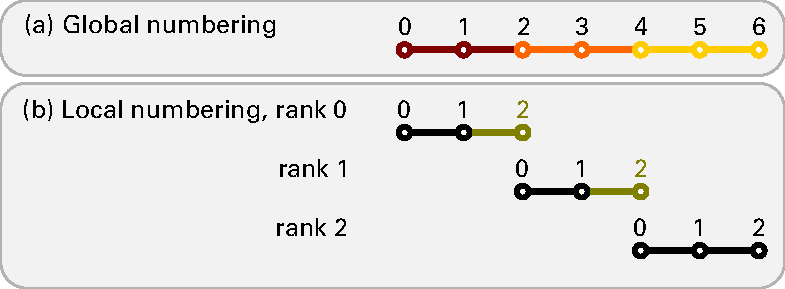
\includegraphics[width=0.6\textwidth]{images/implementation/1d_nodes.pdf}%
  \caption{Partitioning and local and global numbering of a 1D mesh with $N^\text{el}_x=6$ elements partitioned to $n_x=3$ processes. Ghost nodes are marked in green in (b)}%
  \label{fig:1d_nodes}%
\end{figure}%

%2D dof numbering local and global
\begin{figure}%
  \centering%
  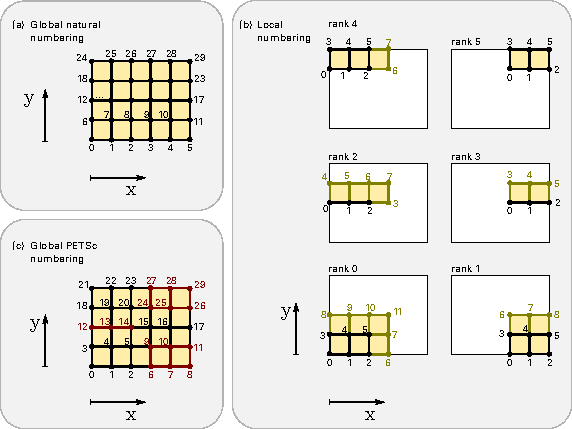
\includegraphics[width=\textwidth]{images/implementation/dof_numbering.pdf}%
  \caption{Subdomains and numberings of a 2D mesh with $N^\text{el}_x \times N^\text{el}_y=5\times 4$ elements partitioned to $n_x\times n_y = 2 \times 3$ processes. (a)-(c) show the different numberings needed for (a) boundary condition specification, (b) identification of local non-ghost dofs (black) and local ghost dofs (green), and (c) identification of global dofs.}%
  \label{fig:dof_numbering}%
\end{figure}%

\renewcommand{\Vec}{\code{Vec}}

On the partitioned meshes, field variables can be defined to represent the scalar and vector fields in the FEM computations. A field variable in \opendihu{} manages its values using the basic PETSc data type for storing scalar fields: the \emph{\Vec{}}. It represents a vector $\tilde{\bfv} \in \R^{n_\text{global}}$ with $n_\text{global}$ values. The vector is distributed to $n_\text{proc}$ processes according to the partitioning of the mesh, such that every value is owned by exactly one process. 

In a PETSc \Vec{}, every rank $r$ locally stores a distinct portion of $n_\text{local\_without\_ghosts} \leq n_\text{global}$ values of the global vector of dofs. Therefore, every dof is \emph{owned} by exactly one rank. These dofs correspond to the local nodes in the partitioning.
Additionally, the process maintains storage for $n_\text{ghosts}$ ghost dofs that are owned by other ranks. 
%Again, the ghost dofs correspond to the ghost nodes of the partitioning. 
PETSc is able to communicate corresponding values between all ranks where the dof is present either as ghost or non-ghost dof. 

In total, the local buffer of a \Vec{} stores $n_\text{local\_with\_ghosts} = n_\text{local\_without\_ghosts} + n_\text{ghosts}$ values. The non-ghost dofs are located at array positions $0,\dots,n_\text{local\_without\_ghosts}-1$, the ghost dofs follow at positions $n_\text{local\_without\_ghosts}, \dots, n_\text{local\_with\_ghosts}-1$. This array is consecutive in memory. The latter part for the ghost dofs is called the \emph{ghost buffer}. 

The local dofs in every subdomain are numbered according to the layout of this buffer. \Cref{fig:1d_nodes} (b) shows the local dof numbering on the three ranks. It proceeds through all non-ghost dofs followed by the ghost dofs. A global numbering of all dofs is given in \Cref{fig:1d_nodes} (a). It is needed, if global operations have to be performed with the \Vec{}, e.g., computing matrix vector products.

In the following, we outline how the finite element stiffness and mass matrices are assembled in parallel.
The algorithm proceeds by iterating over the elements of the mesh. The contributions to the matrix, i.e., the \say{element matrices}, are computed at the dofs of every element. 
Additional material data, such as values of a diffusion tensor, may be stored at the dofs and are used in these computations.

The step of assembling the global matrix entries adds up the contributions of all elements that are adjacent to every dof.
This includes a parallel reduction operation for the ghost dofs, which contribute to matrix entries that are owned by a different subdomain.

% Petsc ghosts, Petsc communication functions
PETSc provides specific functionality for the two required communication operations: (i) gathering data into the ghost buffers on every rank, i.e., communicating the values from the owning rank to the ghost buffers at all other ranks, where the respective dofs are ghosts, and (ii) the global reduction of values between ghost and non-ghost dofs, i.e., communicating the values from the ghost buffers back to the one rank, where they are non-ghosts and adding their values to the values present at the respective rank.

%First, communicating the values from the owning rank to the ghost buffers at all other ranks where the respective dofs are ghosts. 
%Second, . \Cref{fig:1d_comm1} and \cref{fig:1d_comm2} visualize the data flow in the two operations. 

\begin{figure}%
  \centering%
  \begin{subfigure}[t]{0.45\textwidth}%
    \centering%
    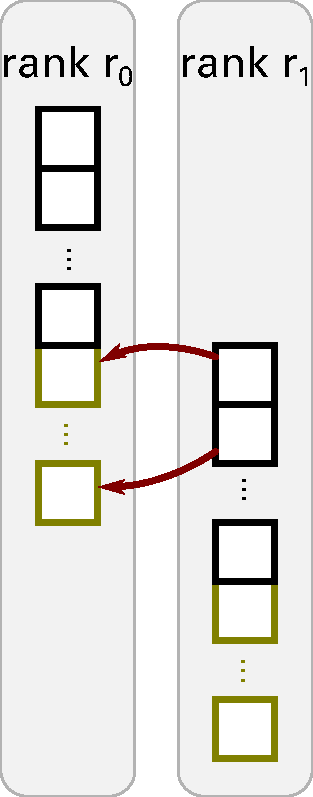
\includegraphics[height=6cm]{images/implementation/1d_comm1.pdf}
    \caption{\code{startGhostManipulation()}: Communication of values at $r_1$ to the ghost buffer at $r_0$.}%
    \label{fig:1d_comm1}%
  \end{subfigure}
  \quad
  \begin{subfigure}[t]{0.45\textwidth}%
    \centering%
    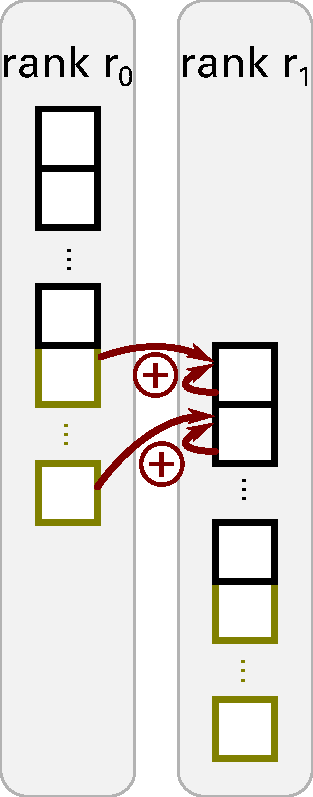
\includegraphics[height=6cm]{images/implementation/1d_comm2.pdf}
    \caption{\code{finishGhostManipulation()}: Communication and addition of ghost values at $r_0$ to the non-ghost dofs at $r_1$.}%
    \label{fig:1d_comm2}%
  \end{subfigure}
  \caption{Communication operations for ghost values in an example with two ranks $r_0$ and $r_1$. Depicted are the vectors of local storage for non-ghost (black) and ghost values (green). The red arrows indicate the data transfer. The visualized operations are needed, e.g., in the assembly of finite element stiffness and mass matrices and their application on the vector of unknowns.}%
  \label{fig:1d_comm}%
\end{figure}%
The \opendihu{} code wraps the two operations in the methods \code{startGhostManipulation()} and \code{finishGhostManipulation()}. After the call to \code{startGhostManipulation()}, the vector can be accessed using the local dof numbering. Values of the local dofs including ghosts can be retrieved, inserted or added as needed, e.g., during FEM matrix assembly. 
After a concluding call to \code{finishGhostManipulation()}, the vector is in a valid global state. Then, global operations such as adding or scaling the whole vector, computing a norm or a matrix vector product can be performed by using the respective PETSc routines. For these operations, the partitioning is transparent, i.e., the calls are the same for serial and parallel execution. Individual entries of the vector can now be accessed using a global numbering. However, every process can still only access the non-ghost dofs owned by its subdomain. The two operations can be interpreted as switching between a local and a global view on the vector object.

One thing to note is that calling \code{startGhostManipulation()} and \code{finishGhostManipu-}\\\code{lation()} directly in sequence changes the values of the vector. The reason is that during the call to \code{startGhostManipulation()}, the ghost buffers get filled with the ghost values from other subdomains. Then, by \code{finishGhostManipulation()} the values in every ghost buffer get summed up and added to the value at the corresponding non-ghost dof. Thus, these dof values finally have a multiple of their initial value.  This is usually not intended. Thus, between the calls to the two methods either all ghost values have to be set, such as during computation of the stiffness matrix. Or, if the ghost values were only needed for reading instead of updating them, the ghost buffers have to be cleared to zero. For the latter, a helper method \code{zeroGhostBuffer()} exists. A typical usage is therefore to call \code{startGhostManipulation()}, then operate on the local dof values including ghosts, and then finish with \code{zeroGhostBuffer()} and \code{finishGhostManipulation()}.


\subsection{Numbering Schemes for Nodes and Degrees of Freedom}\label{sec:numbering_schemes_for}

% partitioned 2D vector, domain numbering, for structured grid with linear ansatz functions
PETSc's definition of the local value buffer used by \Vec{} objects dictates the local numbering scheme of dofs on meshes of any dimensionality. While, for 1D meshes, the numbering as given in \cref{fig:1d_nodes} seems natural, for 2D and 3D meshes, a more complex ordering of local dofs is needed.

Three different numbering schemes for nodes and dofs exist within \opendihu{}. They are visualized in \cref{fig:dof_numbering} for a 2D mesh. The first is the \emph{global natural} numbering scheme, which numbers all $n_\text{global} = N^\text{dofs}_x \times N^\text{dofs}_y \times N^\text{dofs}_z$ global dofs in the structured mesh. It starts with zero and iterates through the mesh using the triple of coordinate indices $(i,j,k)$ for the $x$, $y$ and $z$ axis with the ranges $i \in \{0,\dots,N^\text{dofs}_x-1\}$, $j \in \{0,\dots,N^\text{dofs}_y-1\}$ and $k \in \{0,\dots,N^\text{dofs}_z-1\}$. The numbering proceeds fastest in $x$ or $i$ direction, then in $y$ or $j$ direction and then in $z$ or $k$ direction. Examples are shown in \cref{fig:dof_numbering} (a) for a 2D mesh  and in \cref{fig:dof_numbering_global_3D} for a 3D mesh.

The intention of this first numbering is to facilitate the problem description by the user. If values for a variable in the whole computational domain should be specified, the order of the given value list will be interpreted according to this numbering. Boundary conditions can be given for some dofs by simply specifying the corresponding dof numbers in global natural numbering. The advantage is that this numbering scheme is easily understandable from a users' perspective and independent of the partitioning.

The second numbering scheme is the \emph{local} numbering. An example is given in \cref{fig:dof_numbering} (b). It specifies the order of dofs in the local PETSc \Vec{} and is defined locally on every subdomain for the non-ghost and ghost dofs. At first, all non-ghost dofs are numbered with the order equal to the one in the global natural scheme. Then, all ghost dofs are numbered, again in the order of the global natural scheme. This numbering has the counter-intuitive property of jumps between some neighboring nodes.

The third numbering scheme is called \emph{global PETSc} numbering and is defined by PETSc. It is the numbering used to access global \Vec{}s. It is also the ordering of the rows and columns of matrices. The numbering starts with all local non-ghost numbers on rank 0, then proceeds over all non-ghost numbers of rank 1 and continues like this for all remaining ranks. An example for this numbering is given in \cref{fig:dof_numbering} (c). The portions of local dofs for the different ranks are indicated by the grid of red and black colors. This numbering depends on the partitioning and, thus, on the number of processes. For serial execution it is identical to the global natural numbering.

\begin{figure}%
  \centering%
  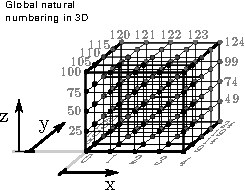
\includegraphics[width=0.5\textwidth]{images/implementation/dof_numbering_global_3D.pdf}%
  \caption{Global natural numbering of nodes in a mesh with $4 \times 4 \times 4$ linear elements.}%
  \label{fig:dof_numbering_global_3D}%
\end{figure}%

\subsection{Parallel Data Structures in \Opendihu{}}\label{sec:paralel_data_structures_in_opendihu}

All operations on scalar and vector fields in the simulation break down to manipulating variables of the \Vec{} type provided by PETSc. 
Because this involves low level operations such as working with different numbering schemes and communicating ghost values, an abstraction layer on a higher level is implemented in \opendihu{}. The data handling classes are visualized in \cref{fig:partitioned_petsc_vec} with the data representation in raw memory at the top and increasing abstraction towards the bottom of the figure.

\begin{figure}%
  \centering%
  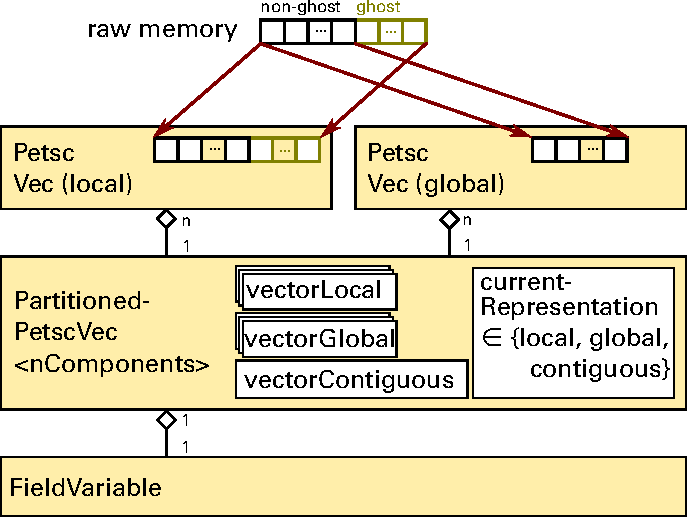
\includegraphics[width=0.8\textwidth]{images/implementation/partitioned_petsc_vec.pdf}%
  \caption{Classes in \opendihu{} that represent vectors in parallel execution. The abstraction layer increases from raw memory at the top to the \code{FieldVariable} at the bottom.}%
  \label{fig:partitioned_petsc_vec}%
\end{figure}%

Depending on whether the local or the global PETSc numbering scheme describes the data, two different objects of the \Vec{} type are used: one local and one global \Vec{}. In \cref{fig:partitioned_petsc_vec}, these two \Vec{}s are represented by the \emph{PETSc Vec (local)} and \emph{PETSc Vec (global)} boxes. At any time, only one of these is in a valid state and allows to manipulate the data. Internally, both PETSc \Vec{}s use the same memory to store their data. However, as shown at the top of \cref{fig:partitioned_petsc_vec}, the memory range of the local \Vec{}'s buffer includes the ghost buffer, which is never accessed by the global \Vec{}. As mentioned, PETSc functions are available to switch the valid state between the two \Vec{}'s, involving communication of ghost values. 
%Because of the shared memory, no costly value copy operation is needed for this action.

The next abstracting class is \emphcode{PartitionedPetscVec<nComponents>}. It represents a discretized vector field $\bfv : \Omega \to \R^c$ with a given number of components $c$. The number of components $c$ is a template parameter to the class, which has to be specified at compile time. 
An example for such vector fields is the \emph{geometry field} with $c=3$, which is defined for every mesh and specifies the node positions. Another example is the solution variable of the considered problem. For scalar problems such as the Laplace equation, it has $c=1$ component, for vector-valued problems, e.g., static elasticity, it has $c=3$ components, namely the displacements in $x$, $y$ and $z$ direction. For the subcellular model of Shorten \cite{Shorten2007}, the solution variable, i.e., the vector of states has $c=57$ components.

For each component, a separate pair of local and global \Vec{}s is stored in the variables \emphcode{vectorLocal} and \emphcode{vectorGlobal}. The global number of entries in each of the \Vec{}s is given by the number $n_\text{global}$ of dofs in the mesh that discretizes the domain $\Omega$. Thus, the memory layout of such a multi-component vector is struct-of-array (SoA). 

Besides \code{vectorLocal} and \code{vectorGlobal}, a third variable \emphcode{vectorContiguous} of type \Vec{} exists in the class \code{PartitionedPetscVec}. It contains the concatenated values of all component vectors in \code{vectorGlobal}. Its size is therefore $c\cdot n_\text{global}$ and the layout is again SoA but stored in a single \Vec{}.

This representation is chosen when a timestepping scheme operates on a state vector with multiple components. An example is the solution of multiple instances of a subcellular problem. Here, the dofs in the mesh correspond to the individual instances and the components are the state variables of the system of ODEs. Thus, the contiguous vector begins with the values of the first state for all instances, then stores the values of the second state for all instances, etc. If the right-hand side of the system of ODEs is evaluated together for all instances, this memory layout is very efficient as it leads to a cache aware access pattern.

Only one of the three vectors \code{vectorLocal}, \code{vectorGlobal} and \code{vectorContiguous} is valid at any time and can be used to retrieve or update the vector values. 
A state variable \emphcode{currentRepresentation} in \code{PartitionedPetscVec<nComponents>} indicates which one that is. The state and the \Vec{} variables are encapsulated and hidden in the class, i.e., not directly accessible from outside. Instead, the class provides data access methods and ways to change the internal representation. For example, calls to \code{startGhostManipulation()} and \code{finishGhostManipulation()} change the representation from global to local and from local to global, respectively.
Thus, it is ensured that only the current valid representation gets accessed at any time.

As noted before, the change between local and global representation does not involve data copying because of the shared physical data structures.
When the representation is changed from local to contiguous, the $c$ sets of values of the \code{vectorLocal} variables have to be copied into the buffer of \code{vectorContiguous}. This operation is performed by copying memory blocks  \mbox{(\code{memcpy})} instead of the slower iteration over all values and the value-wise copy. The reverse change from contiguous back to local representation happens analogously. Thus, the change between all representations is fast. Despite occurring often during transient simulations, profiling of simulations has shown negligible runtime for the action of switching between these representations.

The top level class in the value storage hierarchy as shown in \cref{fig:partitioned_petsc_vec} is the \emphcode{Field Variable}, which contains a \code{PartitionedPetscVec} and adds numerous methods to facilitate access to the data container. Model formulations use this class to manipulate scalar and vector fields. At the same time, the underlying global PETSc \Vec{} can still be obtained from a \code{FieldVariable}. Vector operations such as addition, norms and matrix-vector products are performed using the low-level PETSc functions on the global \Vec{} obtained from the \code{FieldVariable}s.

\subsection{Discussion of Several Design Decisions}
% design decision compile time c and separate vectors, comparison with OpenCMISS iron
In the following, some of the design decisions in \crefrange{sec:oragnization_of_parallel_partitioned_data}{sec:paralel_data_structures_in_opendihu} are discussed.
% numbering, not using DMDA
In the present code, PETSc functionality is used for value storage and organization of ghost values transfer. 
The employed PETSc data model naturally corresponds to a 1D mesh.
The representation of arbitrary dimensional meshes is added by \opendihu{} and involves the presented local and global PETSc numberings. 

PETSc also provides the management of abstract 2D and 3D mesh objects in the \code{DM} (data management) module. It allows to automatically create a partitioning with local numberings and data vectors. However, the mesh always has a symmetric ghost node layout, where ghost layers are present on all faces of a subdomain (box stencil) or also at diagonal neighbors (star stencil). This partitioning layout is based on distributing the nodes of the mesh to all processes. It is needed, e.g., for Finite Difference computations. For the finite element method, however, we need an element based partitioning with ghost layers only on one end of the mesh per coordinate direction. Therefore, we do not use this functionality of PETSc and instead implemented the numberings for 2D and 3D meshes on our own.

% layout with multiple vectors, not one long vector
Another choice was made regarding the data layout in the \code{PartitionedPetscVec} class. Instead of an interleaved storage of the component values in one long \Vec{} in array-of-struct (AoS) memory layout, one separate \Vec{} for each component is stored, which corresponds to SoA layout. 
%The reason for this is better performance as discussed earlier. 
Thereby, the implementation differs from OpenCMISS Iron, which is also based on PETSc, but uses the AoS  approach. 

In Iron, not only the values of multiple components, but actually the values of multiple field variable are combined into a single \Vec{}. A local numbering is defined that enumerates all components, all dofs, and all field variables. Differences to our code are, that Iron uses unstructured meshes, which additionally are allowed to contain different types of elements in a single mesh. Field variables can be defined with dofs either  associated with nodes or with elements. 
All these possible variations are accounted for by the local numbering. 
The construction of the numbering is, thus, a complex process. Iron implements it by a loop over all $n_\text{global}$ dofs of the domain. The same loop is executed in parallel by all $n_\text{proc}$ processes. The runtime complexity of this approach is $\O(n_\text{global})$ regardless of the partitioning. 
In contrast, \opendihu{} constructs its local numberings separately on each process and only iterates over the $n_\text{local\_with\_ghosts}$ dofs, leading to a runtime complexity of $\O(n_\text{local\_with\_ghosts}) = \O(n_\text{global} / n_\text{proc})$. In a weak scaling experiment with constant relation $n_\text{global} / n_\text{proc}$, the approach of Iron yields infinite runtime in the limit for $n_\text{global} \to \infty$, whereas the runtime in the approach of \opendihu{} stays constant.

For \opendihu{}, the AoS approach with separate \Vec{}s was chosen for three reasons. First, it is more cache efficient than the alternative during the computation of the subcellular model, as explained in \cref{sec:paralel_data_structures_in_opendihu}.

Second, the AoS structure is easier, and it allows to treat the components separately, which makes modular code possible. Only a single local dof numbering has to be constructed per mesh, and it can be reused for all components of all field variables.

Third, it is possible to extract one component of a vector-valued field variable and place it into another, scalar field variable without copying. This is used during the solution of the monodomain equations given in \cref{eq:monodomain}. There, the subcellular models have a vector-valued solution variable and the diffusion problem needs a scalar solution variable that consists of the first component of the vector-valued variable of the subcellular model. This first component is the transmembrane voltage $V_m$. The program needs to switch between these two required vectors in every timestep of the splitting scheme. Only with the chosen representation by multiple \Vec{}s, the \Vec{} for the particular component can be efficiently exchanged between the two field variables without an expensive copy operation.

% nComponents compile time
Another design decision was to make the number $c$ of components fixed at compile time. 
Upon construction of a new \code{FieldVariable}, its number of components needs to be known. Typically, this is the case and does not pose any restriction.
The main advantage is that local variables that hold all components for a given dof can be allocated on the stack instead of a much slower dynamic allocation on the heap. For example, in a dynamic solid mechanics problem, the solution \code{FieldVariable} contains three components each for displacements and velocities plus one component for the pressure, in total $c=7$ components. The program can use static arrays with seven entries as temporary variables to handle these values in various computations. If the number of components was not fixed at compile time, a costly dynamic allocation of the seven components would be needed wherever values of the \code{FieldVariable} are retrieved. 
In addition, with a compile-time fixed $c$ the compiler knows the size of the arrays and can perform automatic optimizations such as vectorization and loop unrolling.

The C++ implementation of \code{FieldVariable}s and all other constructs that depend on the number of components is generic, as the  $c$ value is a template argument. Specializations for particular numbers of components such as for the scalar case $c=1$ are possible using \emph{template specialization}.
This flexibility while using object orientation is an advantage over codes using procedural programming languages such as the Fortran standard used by OpenCMISS Iron. It contributes to the extensibility design goal of \opendihu.

\subsection{Implemented Basis Functions}
% different mesh types and ansatz functions, numberings

In the FEM, the number of dofs and nodes per element depends on the chosen ansatz functions or basis functions. \Opendihu{} supports linear and quadratic Lagrange as well as cubic Hermite basis functions. 
\Cref{tab:ansatz_functions_mesh} shows these three sets of functions and the resulting node configuration of an element in a 1D, 2D and 3D mesh.
Profiling showed that evaluation of the basis functions contributes most to the runtime during calculation of the stiffness matrix. Therefore, care was taken to choose the formulations of the basis functions among different factorizations that need the least operations. Those are listed in \cref{tab:ansatz_functions_mesh}.

\begin{table}
  \centering%
  \begin{tabular}{|ll|lll|}
    \hline
    \multicolumn{2}{|l|}{Ansatz functions} \hspace*{43.82mm} & \multicolumn{3}{l|}{Element shapes}  \\
                                         && 1D \hspace*{11mm} & 2D \hspace*{11mm}& 3D\hspace*{11.75mm}\\
    \hline
  \end{tabular}
  \begin{tabular}{|ll|lll|}
    \vspace*{-5mm}
      &&&&\\
      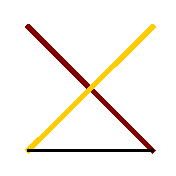
\includegraphics[width=2cm]{images/implementation/ansatz1.pdf}&
      \begin{minipage}{5cm}
        \vspace{-2cm}
        $\phi_0(\xi) = 1-\xi$,\\[2mm] 
        $\phi_1(\xi) = \xi$
      \end{minipage}
       &
      
\includegraphics[width=15mm]{images/implementation/ansatz_mesh_1.pdf} & 
      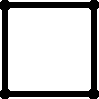
\includegraphics[width=15mm]{images/implementation/ansatz_mesh_2.pdf} &
      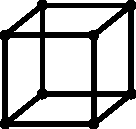
\includegraphics[width=2cm]{images/implementation/ansatz_mesh_3.pdf} \\
    \hline
      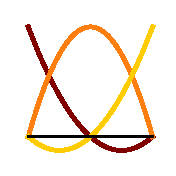
\includegraphics[width=2cm]{images/implementation/ansatz2.pdf}&
      \begin{minipage}{5cm}
        \vspace{-15mm}
        $\phi_0(\xi) = (2\,\xi - 1) \,(\xi-1), $ \\[2mm]
        $\phi_1(\xi) = 4\,(\xi - \xi^2),$    \\[2mm] 
        $\phi_2(\xi) = 2\,\xi^2 - \xi$
      \end{minipage}
       &
      
\includegraphics[width=15mm]{images/implementation/ansatz_mesh_4.pdf} & 
      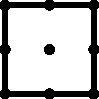
\includegraphics[width=15mm]{images/implementation/ansatz_mesh_5.pdf} &
      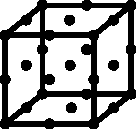
\includegraphics[width=2cm]{images/implementation/ansatz_mesh_6.pdf} \vspace{2mm}\\
    \hline
      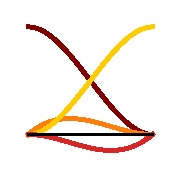
\includegraphics[width=2cm]{images/implementation/ansatz3.pdf}&
      \begin{minipage}{5cm}
        \vspace{-1cm}
        $\phi_0(\xi) = 2\,\xi^3- 3\,\xi^2 + 1, $\\[2mm]
        $\phi_1(\xi) = \xi\,(\xi-1)^2,         $\\[2mm]
        $\phi_2(\xi) = \xi^2 \, (3 - 2\,\xi),  $\\[2mm]
        $\phi_3(\xi) = \xi^2 \, (\xi-1)  $
      \end{minipage}
       &
      
\includegraphics[width=15mm]{images/implementation/ansatz_mesh_1.pdf} & 
      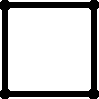
\includegraphics[width=15mm]{images/implementation/ansatz_mesh_2.pdf} &
      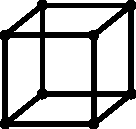
\includegraphics[width=2cm]{images/implementation/ansatz_mesh_3.pdf} \vspace{2mm}\\
    \hline
  \end{tabular}
  \caption{Finite element ansatz functions and resulting element shapes of hexahedral meshes in 1D, 2D and 3D. From top to bottom: Linear Lagrange, quadratic Lagrange and cubic Hermite ansatz functions.}%
  \label{tab:ansatz_functions_mesh}%
\end{table}

In the program, every basis function is defined by a class that specifies the constant, static numbers $n_\text{dofs\_per\_basis}$ of dofs per 1D element and $n_\text{dofs\_per\_node}$ of dofs per node. Furthermore, the actual functions and their first derivatives are implemented. 
All algorithms working with meshes or ansatz functions only use this information given in the basis function class. Therefore, it is easily possible to introduce new nodal ansatz functions as needed, e.g., a cubic Lagrange basis, by accordingly defining a new class.

If any Lagrange basis is used, every node has exactly one dof, i.e., $n_\text{dofs\_per\_node}=1$. With the 1D Hermite basis, every node has $n_\text{dofs\_per\_node}=2$ dofs, one that describes the function value and one that defines the derivative at the particular node. For higher dimensional meshes, the bases are constructed by the tensor product approach. For 2D meshes, this results in four and for 3D meshes in eight dofs per node for the Hermite basis. For example, at a node at location $\bfx$ in a 2D mesh, the first dof describes the value $f(\bfx)$ of a scalar field $f:\Omega \to \R$ and the others relate to the derivatives $\partial_x f(\bfx)$, $\partial_y f(\bfx)$ and $\partial_{xy} f(\bfx)$. 

Note that the dof values for derivatives only match the real derivatives of $f$ in meshes with unity mesh widths. In a general, the derivatives are scaled by the element lengths. In general meshes with varying element sizes, the represented FE solution $f$ is not continuously differentiable at element boundaries, i.e., $f\in\CC^0(\Omega,\R)$.

For quadratic Lagrange and cubic Hermite basis functions, the numbering schemes presented in \cref{sec:numbering_schemes_for} have to be adjusted, such that, at every node, all dofs are enumerated in sequence before the numbering continues at the next node.

\subsection{Implemented Types of Meshes}
Meshes of different types can be selected independently of the choice of basis functions. Three types are supported. \Cref{fig:meshe_types} visualizes meshes of these types with linear and quadratic elements.

The first type is \code{Mesh::RegularFixedOfDimension<D>} where \code{D} $\in \{1,2,3\}$ is a compile-time constant of the dimension. This type describes a rectilinear, regular structured mesh that is defined by a fixed mesh width $h$ in all coordinate directions. This mesh is \say{fixed}, which means that the positions of the nodes cannot change after the mesh object was created. 
Regular fixed meshes describe a line (1D), a rectangular (2D) or a cuboid domain (3D). This mesh type exists, because such domains are often used in exemplary problems to study certain effects independently of the shape of the domain. A regular fixed mesh can be easily configured by specifying origin point coordinates, mesh widths and number of elements. For this mesh type, matrix assembly in the FEM is simplified and more efficient by using precomputed stencils.

\begin{figure}%
  \centering%
  \def\svgwidth{0.5\textwidth}
  \input{images/implementation/meshes.pdf_tex}%
  \caption{The three implemented mesh types in \opendihu{}, each time for 2D linear Lagrange or Hermite ansatz functions (left) and for 2D quadratic Lagrange ansatz functions (right).}%
  \label{fig:meshe_types}%
\end{figure}%

The second mesh type is \code{Mesh::StructuredDeformableOfDimension<D>}. The structured deformable mesh is a generalization of the regular fixed mesh. The mesh again has a structure of $N^\text{el}_x \times N^\text{el}_y \times N^\text{el}_z$ elements. Contrary to the regular fixed mesh, the nodes can now have arbitrary positions. In the name of this mesh, \say{deformable} indicates that the node locations can be changed over time. Thus, this mesh type is usable in dynamic solid mechanics problems, where the domain deforms over time. If the user wants to configure a mesh of this type, they either have to provide the same information as for regular fixed meshes---then, a mesh with fixed mesh width will be created---or they provide the positions of all nodes, yielding an arbitrarily shaped domain as shown in \cref{fig:meshe_types}.

The third mesh type is \code{Mesh::UnstructuredDeformableOfDimension<D>}. In contrast to the two other types, this mesh is unstructured implying that element adjacency is no longer given implicitly.
The example at the lower third of \cref{fig:meshe_types} shows capabilities of this mesh type: The overall shape of the domain is not restricted to resemble a rectangle. Protruding parts like the element at the bottom left are possible. Furthermore, not every node needs to be adjacent to exactly four elements in 2D. The example shows nodes with three and five adjacent elements that allow to properly approximate the round shape of the right side of the domain. The mesh is again \say{deformable}, which means that it can be used for elasticity problems.
In order to configure such a mesh, the node positions have to be specified, similar to a structured deformable mesh. Additionally, the elements with links to their corresponding nodes have to be given.
\Opendihu{} implements a second possibility to specify these meshes. A pair of \code{exelem} and \code{exnode} files, which are common in the OpenCMISS community, can be loaded.

A disadvantage of unstructured meshes is that the simple parallel partitioning scheme of subdividing the domain according to element index ranges is not applicable. Instead, the set of elements for every subdomain needs to be computed individually. Typically, this is done using graph partitioning methods in order to minimize subdomain border lengths while ensuring equal subdomain sizes. Another disadvantage is that information about neighbor elements and neighbor subdomains has to be stored explicitly, while it is given implicitly in structured meshes.
For these reasons, unstructured meshes can be used in \opendihu{} only for serial computation. The construction of parallel partitionings is only possible with the other two, structured mesh types.

The choice, which mesh type to use in a simulation, has to be made at compile time. A simulation program can be easily compiled for different meshes by substituting the type in the main C++ source file.
By proper abstraction in the code, all implemented algorithms are independent of the used mesh type when run in serial. Some algorithms, e.g., streamline tracing, are specialized for structured meshes to exploit the structure and lead to more efficient code. Unit tests ensure the correct solution of a Laplace problem with all combinations of mesh type, dimensionality and ansatz function.

\subsection{Composite Meshes}\label{sec:composite_meshes}

To overcome the limitations of structured meshes regarding possible domain shapes and, at the same time, preserving the advantage of efficient parallel partitioning, \emph{composite} meshes are introduced. These meshes of type \code{Mesh::CompositeOfDimension<D>} are built using multiple meshes of type \code{Mesh::StructuredDeformableOfDimension<D>}, called \emph{submeshes} in this context. The structured submeshes are positioned next to each other to form a combined single mesh on the union of the domains of all meshes. \Cref{fig:meshes_composite} shows a 2D example where three structured meshes are combined to a composite mesh. As can be seen, the submeshes can have different numbers of elements.
The nodes on the borders between touching structured meshes are shared between the individual meshes. Thus, these nodes contain only a single set of dofs like every other node in the mesh.

In the code, composite meshes reuse the implementation of structured meshes by defining different numbering schemes for nodes and dofs over the whole composite domain. The numbering of nodes starts with all nodes of the first submesh, then proceeds over all remaining nodes of the second submesh and so on, until all nodes are numbered. The numbering of dofs is analog. \Cref{fig:dof_numbering_structured_composite} shows an example with two quadratic submeshes with four and two elements. The resulting composite mesh has six elements. The node numbers in the first structured mesh are identical to the corresponding nodes in the composite mesh. The numbering continues in the set of remaining nodes of the second structured mesh and the shared nodes on the border between the meshes are skipped in the numbering, as they already have a number assigned. The shared nodes have the numbers 14, 19 and 24.

In parallel execution, this scheme is executed first on the non-ghost and then on the ghost nodes of the subdomains of all submeshes. Thus, the local numbering of the composite scheme visits the non-ghost nodes of all subdomains first before iterating over the ghost dofs on all subdomains. Thus, the ghost buffer is consecutive in memory as required by the parallel PETSc \Vec{}s.

For the construction of this numbering, the shared nodes of different submeshes, which lie at the same position, have to be determined.
The identification of shared nodes occurs according to their position in the physical domain. The distance in every coordinate direction has to be lower than the tolerance of \num{1e-5} for a pair of nodes to be considered identical and shared. The shared nodes are determined on every local subdomain of the underlying structured meshes. To correctly number ghost nodes that are shared between submeshes, communication between processes is necessary.

Using the set of shared nodes, mappings in both directions between the local numberings of the submeshes and the local and global PETSc numberings of the composite mesh are constructed. These mappings are used to transfer operations on the composite mesh to operations on the structured submeshes. Thus, every implemented algorithm can transparently work also on composite meshes.

The creation of the numbering schemes requires that neighboring elements on different submeshes are located on the same process. If this was not the case, submeshes would potentially have ghost nodes at their outer border, which does not occur in normal structured meshes and would disallow reusing their implementation.
Furthermore, the MPI communicator of the submeshes has to be the same and no subdomain can be empty. This means that a composite mesh has to be partitioned, such that every submesh is subdivided into the same number of partitions involving all processes. If these requirements are fulfilled, the parallel implementation of any algorithm on structured meshes can be reused for composite meshes.
\Cref{fig:meshes_composite} shows a valid partitioning of the exemplary composite mesh to two subdomains.

\begin{figure}%
  \centering%
  \begin{subfigure}[t]{0.45\textwidth}%
    \centering%
    \def\svgwidth{0.7\textwidth}%
    \input{images/implementation/meshes_composite.pdf_tex}
    \caption{A composite mesh that is created from three structured meshes (different colors) and a possible subdivision for parallel partitioning (white vertical line).}%
    \label{fig:meshes_composite}%
  \end{subfigure}
  \quad
  \begin{subfigure}[t]{0.45\textwidth}%
    \centering%
    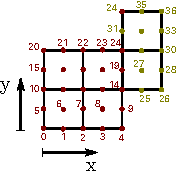
\includegraphics[width=\textwidth]{images/implementation/dof_numbering_structured_composite.pdf}
    \caption{Numbering scheme of dofs for a composite mesh, which is created from two quadratic meshes.}%
    \label{fig:dof_numbering_structured_composite}%
  \end{subfigure}
  \caption{Examples for composite meshes that combine the advantages of structured and unstructured meshes.}%
  \label{fig:composite_meshes}%
\end{figure}%

To configure composite meshes in the settings, their submeshes have to be specified as usual for structured meshes. Then, a list of all submeshes is given for the composite mesh. In parallel execution, a proper partitioning that fulfills the requirements has to be constructed in the Python script of the settings as well.

An application of composite meshes is the biceps muscle with a fat and skin layer. \Cref{fig:composite_muscle_mesh0} visualizes the composite mesh. It consists of two structured submeshes for the muscle belly and the body layer on top, as visualized in the top image. The bottom image shows a partitioning to four processes. As can be seen, the domain can be split along the $x$ and $z$ coordinate axes to produce valid partitionings. Using this decomposition strategy, any number of subdomains (limited by the number of elements, though) is possible.

\begin{figure}%
  \centering%
  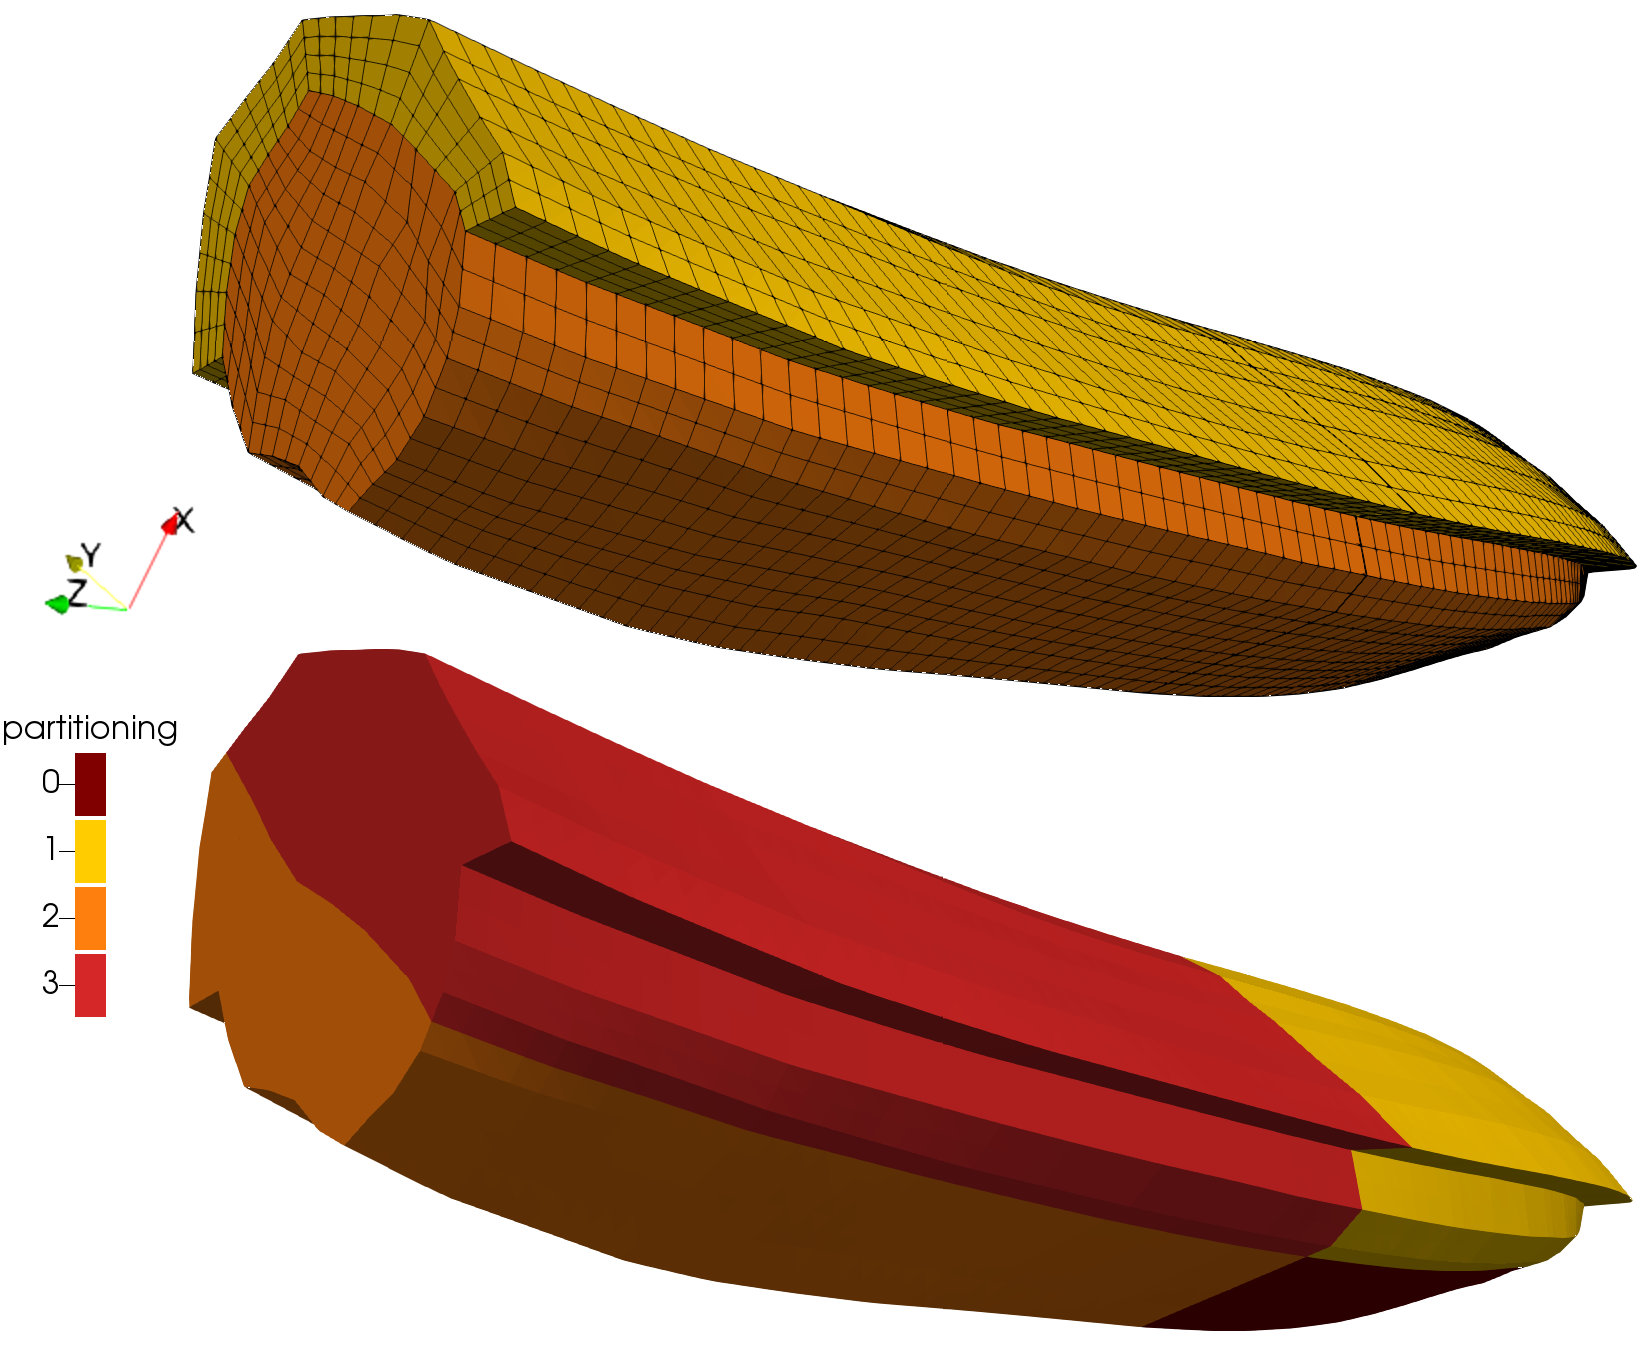
\includegraphics[width=\textwidth]{images/implementation/composite_muscle_mesh0.png}%
  \caption{Composite mesh of the biceps muscle. Top: the two structured meshes from which the composite mesh is created, bottom: partitioning to four processes.}%
  \label{fig:composite_muscle_mesh0}%
\end{figure}%

\section{Finite Element Matrices and Boundary Conditions}\label{sec:fem_matrices_and_bc}
Another important mathematical object besides the vector, which has to be represented in finite element simulation programs, is the matrix. Matrices are mainly needed to store the linear system of equations that results from the discretized weak formulation within the FEM. Dirichlet boundary conditions can be enforced by adjusting the system matrix.

In the following sections, the storage of matrices is discussed, an efficient, parallel algorithm to assemble the FEM system matrix is presented and evaluated and a second parallel algorithm for handling Dirichlet boundary conditions is given.

\subsection{Storage of Matrices}
% matrix storage in Petsc
The storage of matrices is delegated to PETSc, like the storage of vectors. The default sparse  matrix format of PETSc, \emph{compressed row storage (CRS)} or \say{AIJ} in PETSc notion, is used. 
The representation stores the non-zero locations and their values for every row of the matrix.

The system matrices in the FEM have as many rows and columns as there are global dofs in the system. The typical linear system of equations can be expressed as:
\begin{align*}
  \bfK\,\bfu = \bff,
\end{align*}
with system matrix $\bfK$ and the parallel vectors $\bfu$ and $\bff$ of the solution and right-hand side, respectively. The partitioning of the rows of the matrix corresponds to the partitioning of the right-hand side vector $\bff$. Thus, every rank has the complete information of a subset of lines in this matrix equation.

Every rank stores a submatrix of size $n_\text{local\_without\_ghosts} \times n_\text{global}$. In PETSc, this submatrix is composed of two blocks. The \emph{diagonal} block is a square matrix of size $(n_\text{local\_without\_ghosts})^2$ and holds only the columns of the local dofs. The rest of the columns are stored in the \emph{off-diagonal} block which is a non-square matrix in general.

The memory of these two storage blocks needs to be preallocated prior to the assignment of matrix entries. This allows PETSc to allocate the whole data storage in one chunk instead of potential reallocations for every new matrix entry. According to the documentation of PETSc, this can speed up the assembly runtime by a factor of 50 \cite{petsc-web-page}. For the preallocation, the numbers of non-zero entries per row in the two storage blocks need to be estimated. The estimated numbers need to be equal to or greater than the actual number of non-zeros per row.

The stiffness and mass matrices in the FEM have a banded non-zero structure that implies a maximum number of non-zero entries per matrix row. The value can be computed as follows:
\begin{equation}\label{eq:nonzero_estimates}
  \begin{array}{ll}
    n_\text{1D\_overlaps} = (2\,n_\text{dofs\_per\_basis} - 1)\cdot n_\text{dofs\_per\_node},\\[4mm]
    n_\text{non-zeros} = \left(n_\text{1D\_overlaps}\right)^d.
  \end{array}
\end{equation}
Here, the number $n_\text{dofs\_per\_basis}$ of dofs per 1D element is 2 and 3 for linear and quadratic Lagrange bases and 4 for cubic Hermite basis functions. The number $n_\text{dofs\_per\_node}$ of dofs per node is 1 for Lagrange basis functions and 2 for Hermite basis functions. The value $n_\text{1D\_overlaps}$ describes the number of basis functions in a 1D mesh that have overlapping support with a given basis function. By the tensor product approach, the resulting estimate $n_\text{non-zeros}$ of non-zero entries per row is computed by exponentiation of $n_\text{1D\_overlaps}$ with the dimensionality $d$.

Because no assumption can be made about how the bands of non-zero entries in the matrix are distributed to the diagonal and off-diagonal storage parts, the same value of $n_\text{non-zeros}$ is used as estimate to preallocate both the diagonal and the off-diagonal part of the local matrix storage.

In the following, the non-zero structure of an exemplary stiffness matrix is shown. A 3D regular fixed mesh of $4\times 4 \times 4$ elements with quadratic Lagrange basis functions is considered. The Laplace equation is solved with Dirichlet boundary conditions at the bottom and top planes of the volume. The prescribed values are 1 at the bottom and 2 at the top. The solution is visualized in the left of \cref{fig:3d_laplace}. The computation is performed with four processes. \Cref{fig:3d_laplace} shows the partitioning on the right.

\begin{figure}%
  \centering%
  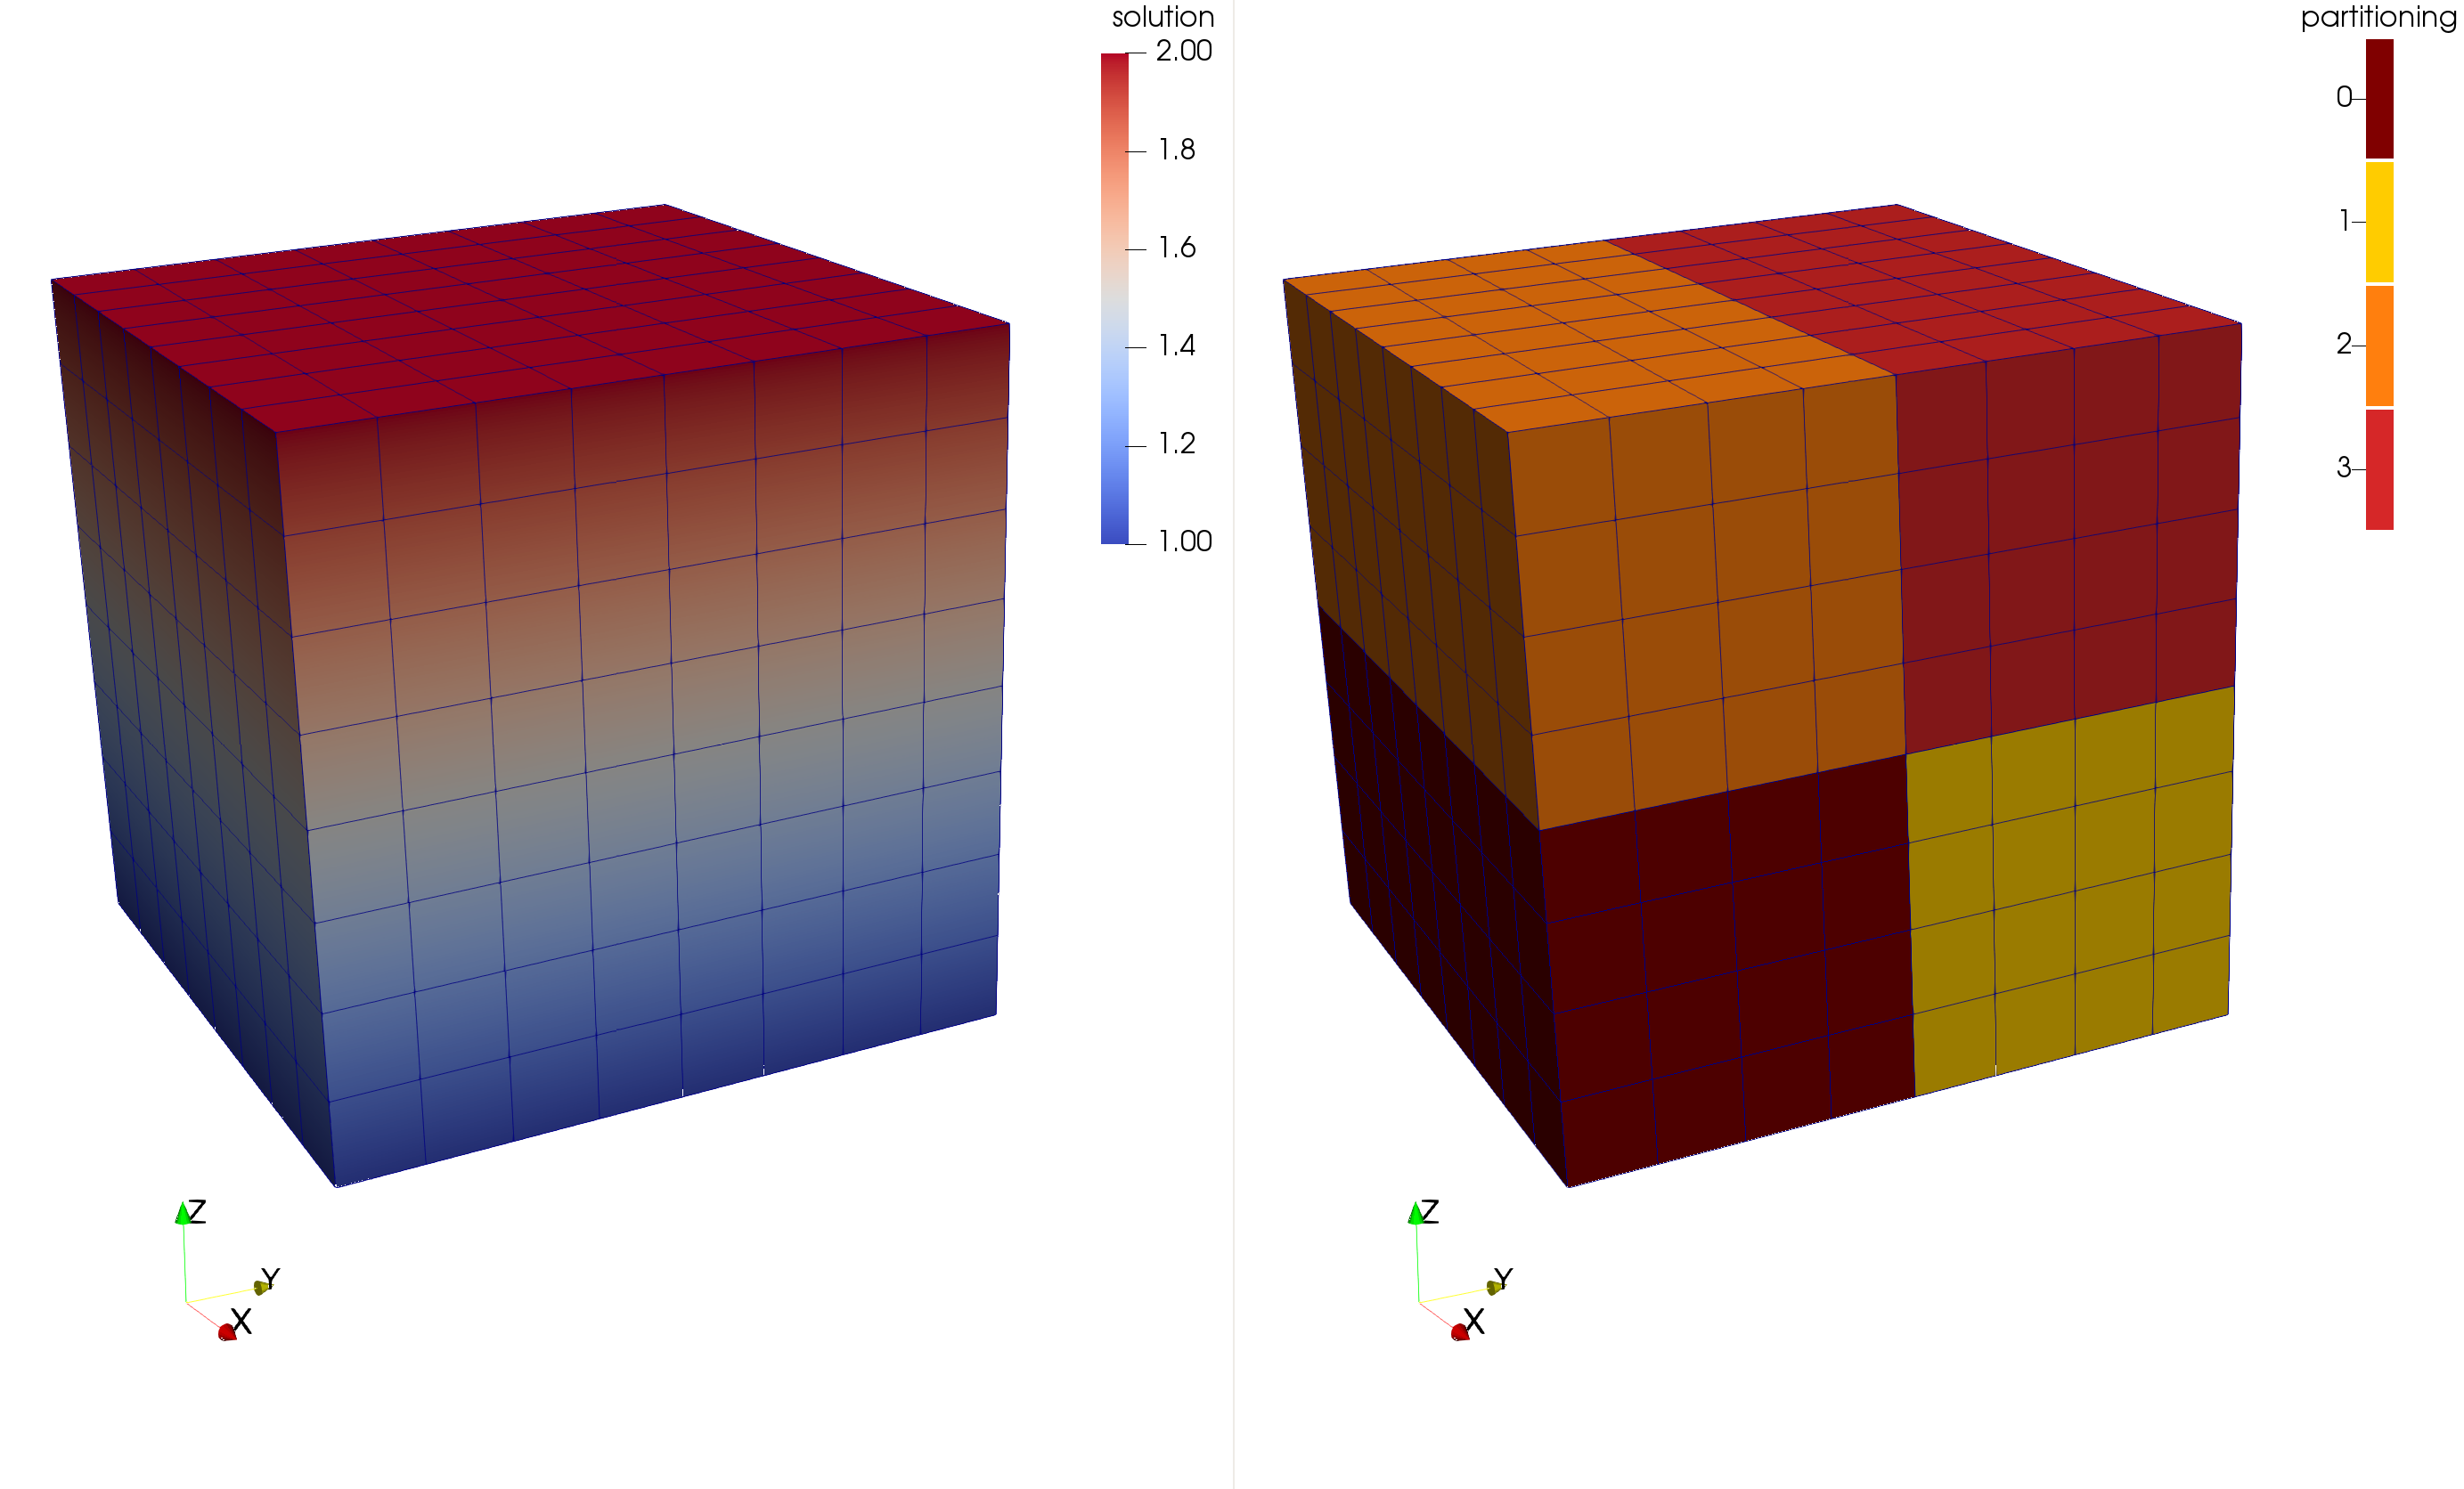
\includegraphics[width=\textwidth]{images/implementation/3d_laplace.png}%
  \caption{Solution of the Laplace equation $ \Delta\bfu = \bff$ with prescribed values $\bfu|_\text{bottom}=1$ and $\bfu|_\text{top}=2.$ The mesh consists of $4\times 4\times 4$ quadratic elements and, thus, $9^3$ nodes. Left: Solution, right: Partitioning to four processes.}
  \label{fig:3d_laplace}%
\end{figure}%

The non-zero estimates computed by \cref{eq:nonzero_estimates} are $n_\text{1D\_overlaps}=5$ and $n_\text{non-zeros} = 125$. The mesh has 4 elements, thus, 9 nodes per coordinate direction, and, therefore, $n_\text{global} = 9^3 = 729$ dofs.
\Cref{fig:sparsity_pattern} shows the resulting sparsity pattern of the stiffness matrix $\bfK$. The portions of the four processes are indicated by different colors. The maximum number of non-zeros per row and column is indeed 125, as calculated. Some rows have less non-zero entries. These correspond to dofs that lie on the boundary of the domain. The rows with only one non-zero entry on the diagonal enforce the Dirichlet boundary conditions. 
The total size of preallocated memory for the diagonal and off-diagonal blocks on all processes is $2\,n_\text{global}\,n_\text{non-zeros} = \num{182250}$. The actual number of non-zero entries is $\num{35937}$, which is approximately $\SI{20}{\percent}$ of the preallocated values.

% This will be explained in more detail in the next section.

\begin{figure}%
  \centering%
  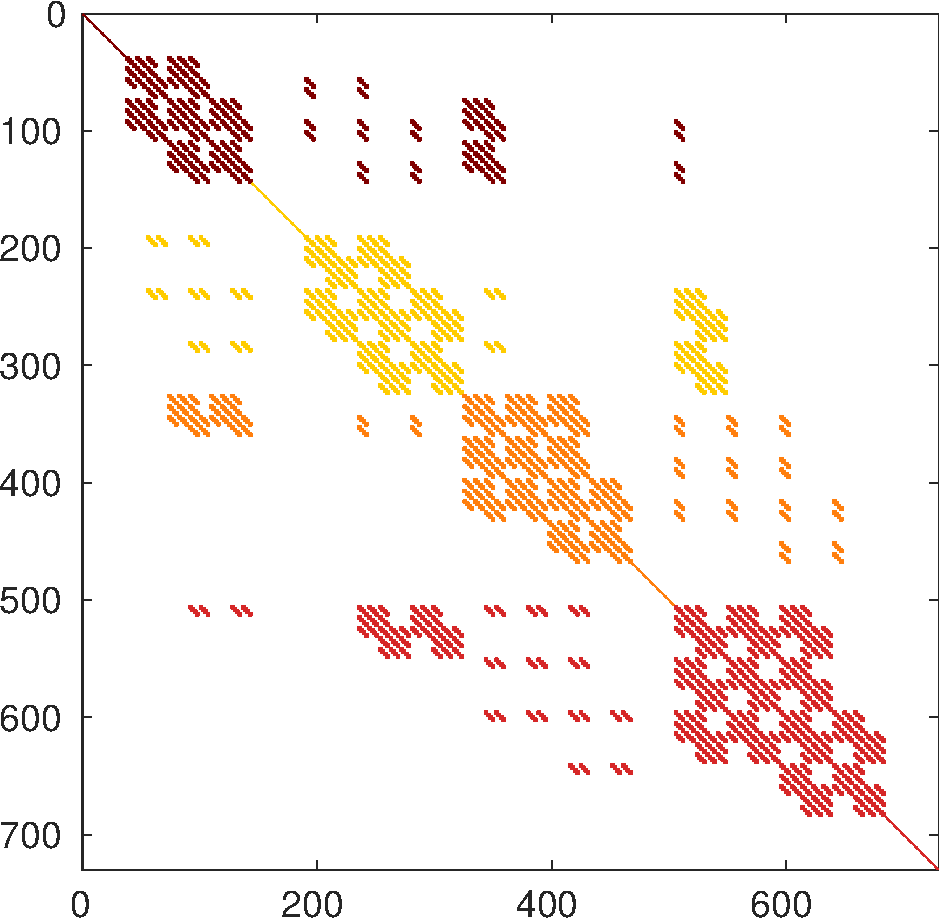
\includegraphics[width=0.7\textwidth]{images/implementation/matrix_sparsity2.pdf}%
  \caption{Sparsity pattern, i.e., locations of non-zero entries of the $729 \times 729$ stiffness matrix $\bfK$ for the example problem in \cref{fig:3d_laplace}. The rows for the four processes are given by different colors matching the partitioning in \cref{fig:3d_laplace}. The processes have 144, 180, 180 and 225 local dofs.}%
  \label{fig:sparsity_pattern}%
\end{figure}%

\begin{reproduce_no_break}
  In any example, the system matrix can be written to a MATLAB compatible file by specifying the settings \code{'dumpFormat': 'matlab', 'dumpFilename': 'out'}.
   %\code{"dumpFormat": "matlab", "dumpFilename": "out"}. 
  To get the non-zero structure for the example in \cref{fig:sparsity_pattern}, compile the \emph{laplace3d} example and run the following:
  \begin{lstlisting}[columns=fullflexible,breaklines=true,postbreak=\mbox{\textcolor{gray}{$\hookrightarrow$}\space}]
    cd $\$$OPENDIHU_HOME/examples/laplace/laplace3d/build_release
    mpirun -n 4 ./laplace_quadratic ../settings_quadratic_matrix_output.py -ksp_view
  \end{lstlisting}
  The flag \code{-ksp\_view} is parsed by PETSc and outputs matrix statistics such as the number of preallocated and actual non-zeros. 
  A file \code{out\_matrix\_000.m} is created that can be loaded in MATLAB. Use \code{spy(stiffnessMatrix)} to plot the non-zero structure.
\end{reproduce_no_break}

\subsection{Assembly of Finite Element Matrices}\label{sec:assembly_of_finite_element_matrices}
% stiffness matrix assembly/integration

Next, the algorithm to compute stiffness and mass matrices in parallel for the application of the $d$-dimensional FEM is discussed.
The matrix entries to be computed are given by%
\begin{align}\label{eq:alg_assembly_m}
  m_{i,j} = \i{\Omega}{} I(\bfx) \,\d\bfx,
\end{align}
where the integrand $I$ is derived from the respective FEM formulation in weak form.

A generic algorithm for the evaluation of this integral and parallel assembly to a global matrix is presented in \cref{alg:fe_matrix_assembly}. Multiple variants of this algorithm, which only differ in their achieved performance, have been implemented for evaluation purposes. They are discussed in \cref{sec:performance_of_the_algorithm_for_pma}. The listed algorithm in \cref{alg:fe_matrix_assembly} shows the fastest variant.

\begin{algorithm}
  \begin{algorithmic}[1]%
    \Procedure{Assemble FE system matrix}{}
    \For{elements $e=\{e_1,e_2,e_3,e_4\}$ in all elements}      \label{line:4.2}
      \For{sampling point $\bfxi$}                              \label{line:4.3}
        \State Compute Jacobian $J_e(\bfxi)$                    \label{line:4.4}
        \State Evaluate integrand $I_{e,i,j}(\bfxi) = c\cdot I(J_e,\bfxi)$ \Comment{for all elements $e$/dofs $(i,j)$ at once}                    \label{line:4.5}
      \EndFor
      \State matrix\_entries[$i$,$j$] = Quadrature($I_{e,i,j}(\bfxi)$)   \Comment{for all el. $e$/dofs $(i,j)$ at once}                    \label{line:4.6}
      
      \For{dof $i$ = $0,\dots,n_\text{dofs\_per\_element}-1$}                      \label{line:4.7}
        \For{dof $j$ = $0,\dots,n_\text{dofs\_per\_element}-1$}                    \label{line:4.8}
          \State rows \hspace*{4.1mm} = dofs $i$ of elements $e_1,e_2,e_3,e_4$                    \label{line:4.9}
          \State columns = dofs $j$ of elements $e_1,e_2,e_3,e_4$  \label{line:4.10}
          \State matrix[rows,columns] = matrix\_entries[$i$,$j$]   \label{line:4.11}
        \EndFor
      \EndFor
    \EndFor
    \State Call PETSc final matrix assembly                    \label{line:4.12}
    \EndProcedure
  \end{algorithmic}%
  \caption{Finite element matrix assembly}%
  \label{alg:fe_matrix_assembly}%
\end{algorithm}%

The main loop in line \algref{alg:fe_matrix_assembly}{line:4.2} iterates over the local elements of the subdomain. 
The shown implementation iterates over sets of four elements $e_1,e_2,e_3$ and $e_4$. A simpler variation of the algorithm is to instead visit every single local element in its own iteration.
However, the more efficient variant is the presented one that always considers the set $e$ of four elements at once. 
Explicit vectorization is employed on all following operations on these four elements, such that 
the four sequences of calculations for the elements are performed by identical instructions. This adheres to the single-instruction-multiple-data (SIMD) paradigm. The vectorization is explicit since the C++ library \emph{Vc} \cite{vc2012,Kretz2015} is used. Vc provides zero-overhead C++ types for explicitly data-parallel programming and directly employs the respective vector instructions where these types are used.

To compute the integral in \cref{eq:alg_assembly_m}, a node based quadrature rule is used. In our code, the quadrature rule has to be chosen at compile time among Gauss, Newton-Cotes and Clenshaw-Curtis quadrature rules. All three schemes are implemented for different numbers $n_\text{sampling\_points}$ of sampling points. The loop in lines \algref{alg:fe_matrix_assembly}{line:4.3}---\algref{alg:fe_matrix_assembly}{line:4.5} iterates over the respective sampling points $\bfxi \in [0,1]^d$ in the element coordinate system. In line \algref{alg:fe_matrix_assembly}{line:4.4}, the Jacobian matrix of the mapping from element to world coordinate frame is computed at the given coordinate $\bfxi$ for all elements in the set $e$. The Jacobian is needed in the integrand for the transformation of the integration domain.

In line \algref{alg:fe_matrix_assembly}{line:4.5}, the integrand $I$ is evaluated for all elements in $e$ and also for all pairs $(i,j)$ of local dofs in each of these elements. The indices $i$ and $j$ are in the range $i,j \in \{0,1,\dots,n_\text{dofs\_per\_element}-1\}$ with the number $n_\text{dofs\_per\_element}$ of dofs per element. The set of $4\,(n_\text{dofs\_per\_element})^2\cdot (n_\text{sampling\_points})^d$ computed values is passed to the implementation of the $d$-dimensional quadrature rule in line \algref{alg:fe_matrix_assembly}{line:4.6}. The numerical values of the integrals get computed for all considered elements in $e$ and dof pairs $(i,j)$, yielding $4\,(n_\text{dofs\_per\_element})^2$ quadrature problems to be solved at once. This means that the result of the quadrature rule is a linear combination of quadrature weights and vector-valued function evaluations instead of scalar function values.

Next, the two loops in lines \algref{alg:fe_matrix_assembly}{line:4.7}---\algref{alg:fe_matrix_assembly}{line:4.11} assign the computed values stored in the variable \code{matrix_entries} to the actual matrix. The loops iterate over all dof pairs $(i,j)$ per element. The corresponding rows and columns are determined in lines \algref{alg:fe_matrix_assembly}{line:4.9} and \algref{alg:fe_matrix_assembly}{line:4.10} and the respective computed value is assigned in line \algref{alg:fe_matrix_assembly}{line:4.11}. 
The values are added to the matrix entry indicated by the row and column index. Since all dofs including ghosts are considered on every local domain, the same matrix entry can get contributions on multiple processes.

Thus, the last step in line \algref{alg:fe_matrix_assembly}{line:4.12} is a PETSc call that communicates and sums all matrix entry contributions to the respective processes where the dof is non-ghost. Additionally, the call frees the residual preallocated memory that was not needed for non-zero entries and finalizes the internal data structure of the CRS storage format.

In the last iteration over local elements of the main loop in line \algref{alg:fe_matrix_assembly}{line:4.2}, the remaining number of elements is potentially less than four. Nevertheless, the computations proceed as normal. The spare entries of the SIMD vectors get computed using dummy values and are discarded at the end.

For the case of vector-valued finite element problems, e.g., linear elasticity with a solution vector of vector-valued displacements, two more inner loops over the components of the vector are inserted. As a result, the presented algorithm can be used to assemble any FEM matrix on any mesh type and for any formulation given by the term $I$ in \cref{eq:alg_assembly_m}.
Examples are stiffness and mass matrices for the Laplace operator with and without diffusion tensor or stiffness and mass matrices for the linear equations that have to be solved during the solution of nonlinear, dynamic elasticity problems.

% algorithms all local, there is no globalToLocal map
Note that the algorithm operates in parallel execution entirely on data stored in the local subdomain and does not need any global information. The loop iterates over local elements. For every element, the indices in the local numbering of the nodes that are adjacent to the element are needed. In structured meshes, this information is determined from the numbers $N^\text{el}_x \times N^\text{el}_y \times N^\text{el}_z$ of local elements in the coordinate directions. In unstructured meshes, these indices are explicitly stored in the elements. To assemble the global matrix, PETSc uses the mapping from local to global numbering, which it can maintain by storing the constant offset in the global numbering on every subdomain. Mappings from global dof or node numbers to local numbers are not needed in this algorithm. 
In general, storing global information, which would require memory of $\O(n_\text{global})$, is avoided in all algorithms to ensure good parallel weak scaling properties.

%A different approach is to iterate over the global matrix entries rather than the elements. Then, 

\subsection{Performance of the Algorithm for Parallel Matrix Assembly}\label{sec:performance_of_the_algorithm_for_pma}

In the following, the performance of two variations of the algorithm in \cref{alg:fe_matrix_assembly} will be examined. The first variation is to not use explicit vectorization and, thus, iterate over the elements one by one instead of the groups of four elements in line \algref{alg:fe_matrix_assembly}{line:4.2}.

The second variation is to not accumulate multiple values for the application of the quadrature scheme in line \algref{alg:fe_matrix_assembly}{line:4.6}. Instead, the loop over the sampling points in line \algref{alg:fe_matrix_assembly}{line:4.3} is made the inner-most loop and placed inside  the loop in line \algref{alg:fe_matrix_assembly}{line:4.8}. Then, the quadrature scheme only computes a single value at once. In consequence, this value can directly be stored in the resulting matrix, and the temporary variable \code{matrix\_entries} is not needed. This loop reordering requires the evaluations of the Jacobian and the integrand in lines \algref{alg:fe_matrix_assembly}{line:4.4} and \algref{alg:fe_matrix_assembly}{line:4.5} to also be located in the new inner-most loop over the sampling points. 

The algorithm with these two variations corresponds to the naive way of implementing matrix assembly because iterating first over elements, then over dof pairs and then performing the quadrature directly mirrors the mathematical description.

Different combinations of these two variations result in four variants of the algorithm. A study was conducted to measure their effects on the runtimes. A simulation with the same settings as in \cref{fig:3d_laplace} was run except for a larger number of $50 \times 50 \times 50$ elements. This setup lead to a total number of $n_\text{global}=\num{1030301}$ dofs. Gauss quadrature with three sampling points per coordinate direction and, thus, $3^3=27$ sampling points in total was used. The program was executed with four processes on an AMD EPYC 7742 processor with base frequency of \SI{2.25}{\giga\hertz}, maximum boost frequency of \SI{3.4}{\giga\hertz}, \SI{2}{\tera\byte} of memory and a memory bandwidth of \SI{204.8}{\giga\byte\per\second} per socket.
The runtime for the assembly of the stiffness matrix with dimensions $n_\text{global} \times n_\text{global}$ was measured for all four variants. \Cref{fig:matrix_runtimes} presents the resulting runtimes.

\begin{figure}%
  \centering%
  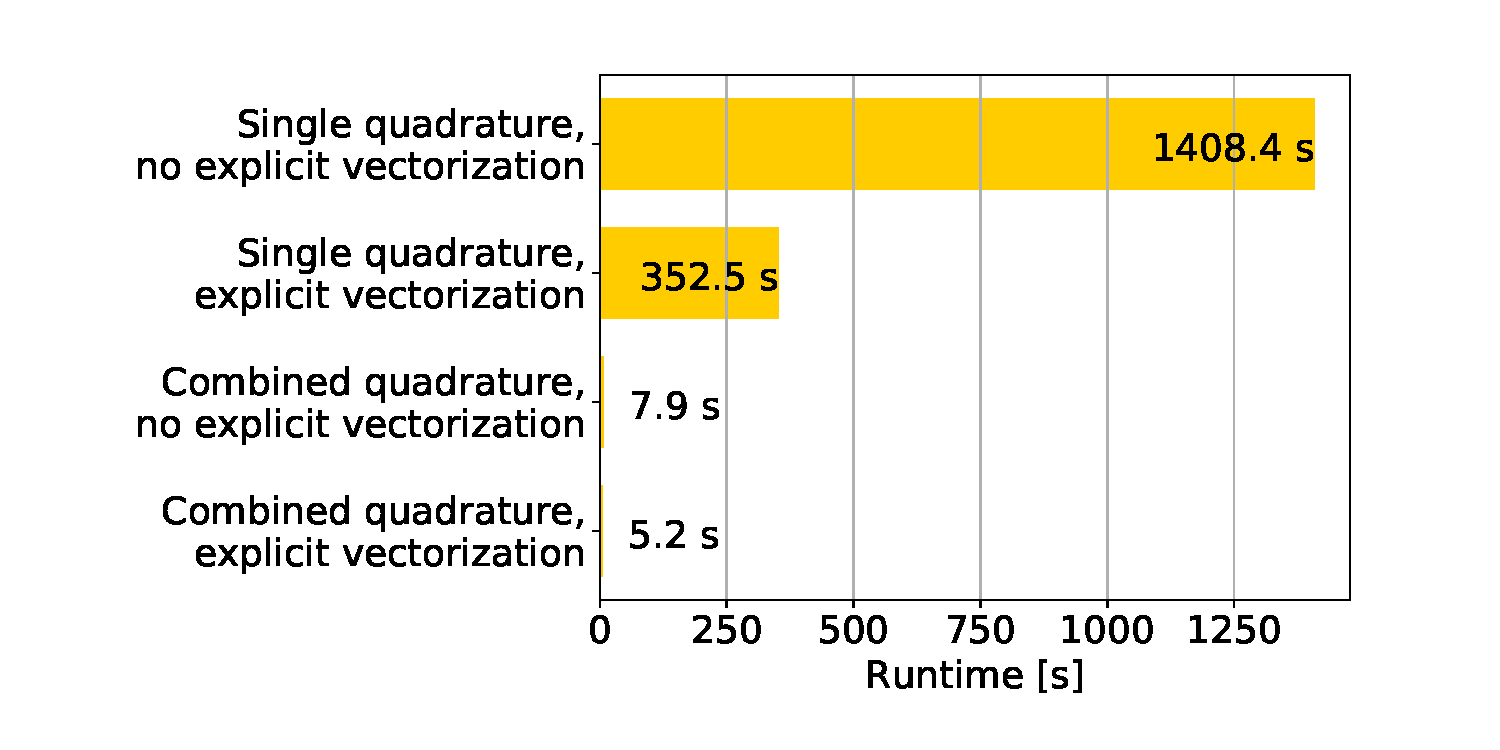
\includegraphics[width=\textwidth]{images/implementation/matrix_runtimes.pdf}%
  \caption{Runtimes of different optimizations for the algorithm to assemble the FEM stiffness matrix.}%
  \label{fig:matrix_runtimes}%
\end{figure}%

It can be seen that a large difference in runtime exists between the variants with quadrature of single values compared to the combined quadrature. In the case of no explicit vectorization (first and third bar from the top in \cref{fig:matrix_runtimes}), the runtime reduces to less than \SI{0.6}{\percent}. In the case of explicit vectorization (second and fourth bar from the top in \cref{fig:matrix_runtimes}), the runtime reduces to less than \SI{1.5}{\percent}. The reason for this enormous gain in performance is three-fold. First, the values of the Jacobian can be reused for the same element and sampling point. Second, the combined quadrature for multiple values yields more cache-efficient memory access, because the vector of values is stored consecutively in memory and can be fetched from the cache by less load operations. For the single quadrature, the individual values are fetched at different times from different memory locations.
Third, the compiler is able to employ SIMD instructions for the combined quadrature, a process called auto-vectorization.

The performance improvements from the second variation, the use of explicit vectorization by simultaneously computing the entries for four elements at once can be seen by comparing the first and second bars and the third and forth bars in \cref{fig:matrix_runtimes}. The runtime reduction of explicit vectorization with single quadrature from \SI{1408.4}{\second} to \SI{352.5}{\second} is exactly by the expected factor of four. This shows that explicit vectorization works as expected, and that no auto-vectorization could be performed by the compiler for the single quadrature. The runtime reduction of explicit vectorization from \SI{7.9}{\second} to \SI{5.2}{\second} during combined quadrature corresponds to a speedup of only approximately \num{1.5}. This shows that combined quadrature without explicit vectorization already allows the compiler to employ some auto-vectorization. However, using the explicit vectorization approach on the level of different elements instead of the level of quadrature values still has a positive effect. 

In total, the performance gain from the most naive implementation (top bar in \cref{fig:matrix_runtimes}) to the most optimized version (bottom bar in \cref{fig:matrix_runtimes}) equals a speedup of more than \num{270}. Together with the solution of the linear system using an algebraic multigrid preconditioner and a GMRES solver with a residual norm tolerance of \num{1e-10}, the total runtime of the program to solve the Laplace problem with over a million degrees of freedom using a modest parallelism of four processes takes \SI{28}{\second}.


\begin{reproduce_no_break}
  The results of \cref{fig:matrix_runtimes} can be reproduced as follows. The explicit vectorization can be turned on and off with the variable \code{USE_VECTORIZED_FE_MATRIX_ASSEMBLY} in the configuration of the SCons build system in the file \code{$\$$OPENDIHU_HOME/user-variables.scons.py} (ca. line 75). Normally, only the variant with combined quadrature is implemented. To test the single quadrature, checkout the git branch \code{fem_assembly_measurement}. The single quadrature is on by default, to change back to the combined quadrature, edit the following line:
  \begin{lstlisting}[columns=fullflexible,breaklines=true,postbreak=\mbox{\textcolor{gray}{$\hookrightarrow$}\space}]
    vi $\$$OPENDIHU_HOME/core/src/spatial_discretization/finite_element_method/01_stiffness_matrix_integrate.tpp +17
  \end{lstlisting}
  For all variants of the algorithm, compile and run the following example: 
  \begin{lstlisting}[columns=fullflexible,breaklines=true,postbreak=\mbox{\textcolor{gray}{$\hookrightarrow$}\space}]
    cd $\$$OPENDIHU_HOME/examples/laplace/laplace3d/build_release
    mpirun -n 4 ./laplace_quadratic ../settings_quadratic.py
  \end{lstlisting}
  The duration of the algorithm for stiffness matrix assembly will be printed.
\end{reproduce_no_break}

% stencils
\subsection{Assembly of Finite Element Matrices for Regular Meshes}

For equidistant meshes of type \code{Mesh::StructuredRegularFixedOfDimension<D>}, all elements are similar through the uniform grid resolution and, thus, all elements matrices equal the same constant matrix. In consequence, the integral terms in \cref{eq:alg_assembly_m} can be precomputed analytically and no numerical quadrature at runtime is needed. This speeds up the determination of the FEM matrices.

We implement matrix assembly using precomputed values for the stiffness and mass matrices of the Laplace operator for linear Lagrange basis  functions. For the stiffness matrix of the Laplace operator, the integral term $(-\int_{\Omega^\text{el}} ∇\phi_i\cdot ∇\phi_j \,\d\bfxi)$ is calculated analytically. The result is a value for every combination of the dofs $i$ and $j$ in the element. 
Thus, the contribution of one representative element in the mesh to the values at adjacent dofs is known. 
To get the matrix entry for a particular dof, the element contributions of all elements that are adjacent to the node need to be summed up. For this process, it is convenient to represent the precomputed values in \emph{stencil notation}.

\Cref{tab:stencils_laplace} shows the stencils for element contributions in the left column and the resulting stencils for the dofs in the right column.
In the element contribution stencils, dof $i$ is chosen as the first dof in the local dof numbering. Values are calculated for all choices of dof $j$ in the element and the values are noted in the stencil. The location of dof $i$ is marked by the underlined number. Stencils for all other locations of dof $i$ follow by symmetry.

The node stencils describe the values of the term $(-\int_{\Omega} ∇\phi_i\cdot ∇\phi_j \,\d\bfxi)$ with the integration over the whole domain. 
The node $i$ is fixed and marked in the stencil notation by the underlined number. Values for all neighboring nodes $j$ are computed and listed in the stencils.
For a given node $i$, the integral over the whole domain $\Omega$ is the sum of integrals over all elements $\Omega^\text{el}$ adjacent to node $i$. These have been computed in the element contribution stencils. As can be seen in \cref{tab:stencils_laplace}, the node stencils follow by adding up mirrored variants of the element stencils centered around the underlined node.

\begin{table}
  \centering
  \begin{tabular}{|c|c|c|c}
      \hline
      Dim. & Element contribution & Node stencil\\
      \hline
      1D &
  \begin{minipage}{4cm}
    \begin{equation*}
       \left[\begin{array}{ccc}
          \underline{-1} & 1\\
      \end{array}\right] \quad 
    \end{equation*}
  \end{minipage} 
      &
  \begin{minipage}{4cm}
    \begin{equation*}
      \left[\begin{array}{ccc}
          1 & \underline{-2} & 1\\
      \end{array}\right]
    \end{equation*}
  \end{minipage} 
       \\[4mm]
       \hline
      2D &
  \begin{minipage}{5cm}
    \begin{equation*}
      \dfrac16\left[
        \begin{array}{ccc}
          1 & 2 \\
          \underline{-4} & 1
        \end{array}
      \right]
    \end{equation*}
  \end{minipage}  &
  \begin{minipage}{5cm}
    \begin{equation*}
        \dfrac13\left[
          \begin{array}{ccc}
            1 & 1 & 1\\
            1 & \underline{-8} & 1 \\
            1 & 1 & 1
          \end{array}
        \right]
    \end{equation*}
  \end{minipage}  \\[4mm]
      \hline
      3D &
  \begin{minipage}{6cm}
    \begin{equation*}
      \begin{array}{ll}
        \text{center:} &
        \dfrac1{12}\left[\begin{array}{ccc}
            0 & 1\\
            \underline{-4} & 0\\
        \end{array}\right] \\[4mm]
        \text{bottom:}& 
        \dfrac1{12}\left[\begin{array}{ccc}
            1 & 1\\
            0 & 1\\
        \end{array}\right]
      \end{array}
    \end{equation*}
  \end{minipage} &
  \begin{minipage}{6cm}
    \begin{equation*}
      \begin{array}{ll}
        \text{top:} &
        \dfrac1{12}
        \left[\begin{array}{ccc}
            1 & 2 & 1\\
            2 & 0 & 2\\
            1 & 2 & 1
        \end{array}\right] \\[4mm]
        \text{center:} &
        \dfrac1{12}
        \left[\begin{array}{ccc}
            2 & 0 & 2\\
            0 & \underline{-32} & 0\\
            2 & 0 & 2
        \end{array}\right] \\[4mm]
        \text{bottom:}& \text{same as top}
      \end{array}  
    \end{equation*}
  \end{minipage}
  \\\hline
  \end{tabular}
  \caption{Stencils of the finite element stiffness matrix of $Δu$ for a regular mesh with mesh width $h=1$ and linear ansatz functions. The stiffness matrix entries can be computed by multiplication with a mesh width dependent factor.}
  \label{tab:stencils_laplace}
\end{table}

\begin{table}
  \centering
  \begin{tabular}{|c|c|c|c}
      \hline
      Dim. & Element contribution & Node stencil\\
      \hline
      1D &
  \begin{minipage}{4.5cm}
    \begin{equation*}
       \dfrac1{6}\left[\begin{array}{ccc}
          \underline{2} & 1\\
      \end{array}\right] \quad 
    \end{equation*}
  \end{minipage} 
      &
  \begin{minipage}{4.5cm}
    \begin{equation*}
      \dfrac1{6}\left[\begin{array}{ccc}
          1 & \underline{4} & 1\\
      \end{array}\right]
    \end{equation*}
  \end{minipage} 
       \\[4mm]
       \hline
      2D&
  \begin{minipage}{5cm}
    \begin{equation*}
      \dfrac1{36}\left[
        \begin{array}{ccc}
          2 & 1 \\
          \underline{4} & 2
        \end{array}
      \right]
    \end{equation*}
  \end{minipage}  &
  \begin{minipage}{5cm}
    \begin{equation*}
        \dfrac1{36}\left[
          \begin{array}{ccc}
            1 & 4 & 1\\
            4 & \underline{16} & 4 \\
            1 & 4 & 1
          \end{array}
        \right]
    \end{equation*}
  \end{minipage}  \\[4mm]
      \hline
      3D &
  \begin{minipage}{6cm}
    \begin{equation*}
      \begin{array}{ll}
        \text{center:} &
        \dfrac1{216}\left[\begin{array}{ccc}
            4 & 2\\
            \underline{8} & 4\\
        \end{array}\right] \\[4mm]
        \text{bottom:}& 
        \dfrac1{216}\left[\begin{array}{ccc}
            2 & 1\\
            4 & 2\\
        \end{array}\right]
      \end{array}
    \end{equation*}
  \end{minipage} &
  \begin{minipage}{6cm}
    \begin{equation*}
      \begin{array}{ll}
        \text{top:} &
        \dfrac1{216}\left[\begin{array}{ccc}
            1 & 4 & 1\\
            4 & 16 & 4\\
            1 & 4 & 1
        \end{array}\right] \\[4mm]
        \text{center:} &
        \dfrac1{216}\left[\begin{array}{ccc}
            4 & 16 & 4\\
            16 & \underline{64} & 16\\
            4 & 16 & 4
        \end{array}\right] \\[4mm]
        \text{bottom:}& \text{same as top}
      \end{array}  
    \end{equation*}
  \end{minipage}
  \\\hline
  \end{tabular}
  \caption{Stencils of the finite element mass matrix for a regular mesh with mesh width $h=1$ and linear ansatz functions. The mass matrix entries can be computed by multiplication with a mesh width dependent factor.}
  \label{tab:stencils_mass_laplace}
\end{table}

The entries in the stiffness matrix are computed from the node stencils by a multiplication with a mesh dependent prefactor.
For 1D, 2D and 3D meshes with mesh width $h$, these prefactors are $1/h$, 1 and $h$, respectively. Thus, e.g., the 1D stiffness matrix has the entries $-2/h$ on the diagonal, $1/h$ on the secondary diagonals above and below the main diagonal and zero everywhere else.

A similar computation is possible for the mass matrix, where the term $\int \phi_i\,\phi_j \,\d\bfxi$ can be precalculated. The element and node stencils for the mass matrix are given in \cref{tab:stencils_mass_laplace}.

The precalculated values can only be used for meshes with uniform mesh width and linear Lagrange basis functions. In \opendihu{}, the type of the mesh and basis function is fixed at compile time. The stencil based approach to set the entries of stiffness and mass matrix is implemented as partial template specialization of the template, which otherwise uses the numerical algorithm presented in \cref{sec:assembly_of_finite_element_matrices}. Thus, the stencil based implementation is instantiated automatically by the compiler for regular fixed meshes of all dimensionalities with linear basis functions. 

The conditions for the stencil based approach are fulfilled whenever regular fixed meshes and linear bases are used, e.g., for toy problems or studies where the shape of the domain is irrelevant and, e.g., a cuboid cutout of muscle tissue is sufficient. Mathematical models involving a Laplace operator, such as Laplace, Poisson or diffusion problems can benefit from the faster system matrix setup.

Another purpose of the stencil based approach in \opendihu{} besides runtime reduction is to verify the implementation of the numerical integration method of \cref{alg:fe_matrix_assembly}. Because of the regular mesh and linear ansatz functions, the numerical method computes the exact result with proper quadrature schemes and, thus, can be compared to the stencil based approach. Several unit tests ensure that the generated system matrices of the two approaches are equal.


\subsection{Algorithm for Dirichlet Boundary Conditions}
% algorithm for Dirichlet boundary conditions

The assembled system matrix needs to be adjusted when Dirichlet boundary conditions are specified.
Dirichlet boundary conditions are ensured by replacing equations involving the prescribed dofs by the definition of the boundary conditions. This involves changes in the system matrix and right-hand side of the finite element formulation.

Consider the following matrix equation resulting from a FE discretization with four dofs $u_1$ to $u_4$:
\begin{equation*}
  \begin{array}{llll}
    \mat{m_{11} & m_{12} & m_{13} & m_{14} \\ m_{21} & m_{22} & m_{23} & m_{24} 
       \\ m_{31} & m_{32} & m_{33} & m_{34} \\ m_{41} & m_{42} & m_{43} & m_{44} }
    \mat{u_1 \\ u_2 \\ u_3 \\ u_4} = \mat{f_1 \\ f_2 \\ f_3 \\ f_4}.
  \end{array}
\end{equation*}
We assume a Dirichlet boundary condition for the last dof, $u_4 = \hat{u}_4$. Enforcing this condition is accomplished by the following adjusted system of equations:
\begin{equation*}
  \begin{array}{llll}
    \mat{m_{11} & m_{12} & m_{13} & 0\\ m_{21} & m_{22} & m_{23} & 0 \\ m_{31} & m_{32} & m_{33} & 0 \\ 0 & 0 & 0 & 1}
    \mat{u_1 \\ u_2 \\ u_3 \\ u_4} 
    = \mat{f_1 - m_{14}\,\hat{u}_4 \\
           f_2 - m_{24}\,\hat{u}_4  \\ 
           f_3 - m_{34}\,\hat{u}_4 \\
          \hat{u}_4}.
  \end{array}
\end{equation*}
The last equation has been replaced by $u_4 = \hat{u}_4$, all summands in the other equations where $u_4$ occurred have been brought to the right-hand side and $u_4$ has been substituted by the prescribed value $\hat{u}_4$.

Thus, setting a dof $u_i$ to a prescribed value $\hat{u}$ corresponds to 
subtracting the column vector of column $i$ of the system matrix multiplied with $\hat{u}$ from the right-hand side, replacing the right-hand side entry at $i$ by $\hat{u}$ and setting row $i$ and column $i$ in the matrix to all zero and the diagonal entry $m_{ii}$ to one.

This method also works for more prescribed values as demonstrated with the additional Dirichlet boundary condition $u_2 = \hat{u}_2$. Executing the scheme results in the following system:
\begin{equation*}
  \begin{array}{llll}
    \mat{m_{11} & 0 & m_{13} & 0\\ 0 & 1 & 0 & 0 \\ m_{31} & 0 & m_{33} & 0 \\ 0 & 0 & 0 & 1}
    \mat{u_1 \\ u_2 \\ u_3 \\ u_4} 
    = \mat{f_1 - m_{12}\,\hat{u}_2 - m_{14}\,\hat{u}_4 \\
          \hat{u}_2 \\ 
           f_3 - m_{32}\,\hat{u}_2 - m_{34}\,\hat{u}_4 \\
          \hat{u}_4}.
  \end{array}
\end{equation*}

During parallel execution, only a distinct subset of rows of the matrix equation is accessible on every rank. 
However, for the subtractions at the right-hand side, the full vector of prescribed boundary conditions values is needed on every rank. Additionally, the corresponding matrix entries are required. While the needed matrix entries are all stored on the local rank, the vector of prescribed values is partitioned to all ranks and only the local subdomain is accessible. 
%However, most of the prescribed values are not needed for the subtraction, because the corresponding matrix entries are zero. 
Some of the non-accessible prescribed values correspond to a non-zero matrix entry, though, and are not needed for the subtraction. In consequence, some data transfer between processes is required. In the following, the identification of the values that have to be communicated is illustrated with an example.

\begin{figure}%
  \centering%
  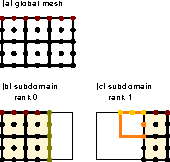
\includegraphics[width=0.6\textwidth]{images/implementation/dirichlet_bc_example.pdf}%
  \caption{Example to illustrate ghost element transfer that is needed for handling Dirichlet boundary conditions in parallel. A mesh with Dirichlet boundary conditions on the red nodes is given in (a). The subdomains for two processes are given in (b) and (c). (c) shows a ghost element in orange that is sent from rank 0 to rank 1.}%
  \label{fig:dirichlet_bc_example}%
\end{figure}%

\Cref{fig:dirichlet_bc_example} (a) shows a 2D quadratic mesh with $3 \times 2$ elements. The top layer of nodes has prescribed Dirichlet boundary conditions, marked by the red circles. The elements are partitioned to two processes with subdomains containing four and two elements, as shown in \cref{fig:dirichlet_bc_example} (b) and \cref{fig:dirichlet_bc_example} (c). 

On rank 0, the right-most layer of nodes consists of ghost nodes. All other nodes are non-ghost and correspond to the matrix rows and right-hand side entries that have to be manipulated by this rank.
In every of these matrix rows $i$, only entries in columns $j$ that correspond to nodes in the same element as $i$ are non-zero. For these columns $j$, the prescribed Dirichlet boundary condition values $\hat{u}_j$ need to be known, such that the product of matrix entry $m_{ij}$ and prescribed value $\hat{u}_j$ can be subtracted from the right-hand side at the corresponding row $i$. This is fulfilled for rank 0 since the required boundary condition values are all part of the subdomain. The top right boundary condition node in the top right element of rank 0's subdomain is stored as ghost value, the other four are non-ghosts.

As can be seen in \cref{fig:dirichlet_bc_example} (c), the subdomain of rank 1 has no ghost nodes. The rank owns three boundary condition nodes in the top layer. It has to perform right-hand side subtractions for the twelve rows of the matrix equation that correspond to the $3\times 4$ other nodes, which have no prescribed boundary condition. For the bottom two horizontal layers of nodes, the subtraction terms are zero, because the bottom element of the subdomain has no boundary conditions and, thus, these matrix entries are all zero.
The upper three horizontal layers of nodes that all belong to the upper element, however, lead to non-zero right-hand side subtraction terms because of the boundary conditions at the top. The terms can be computed for all but the two orange nodes. 
At the corresponding rows $i$, the prescribed values $\hat{u}_j$ for all five yellow and red boundary condition nodes $j$ are needed. However, the left two yellow nodes are not stored on the subdomain of rank 1. They have to be communicated from the subdomain of rank 0. As rank 1 has no topology knowledge of rank 0's subdomain, the information that the missing boundary condition nodes are in the same element as the two orange nodes has to be also transferred. 

In total, the information indicated in \cref{fig:dirichlet_bc_example} (c) by the orange element with the two orange nodes and the three yellow boundary condition nodes and values have to be communicated from rank 0 to rank 1. This element is called \emph{ghost element}.
Rank 0 knows that rank 1 will need this information because it stores the right-most yellow node and the orange nodes in subdomain 1 as ghost nodes in its own subdomain. Therefore, no request from rank 1 is necessary.

In general, every rank constructs ghost elements from own elements that contain both at least one boundary condition node and at least one ghost node without boundary condition. The global indices of all nodes of these two kinds and the corresponding boundary condition values are packaged as ghost element and sent to the rank of the neighboring subdomain. Every process potentially sends multiple ghost elements to multiple neighboring ranks. 

Because a rank does not know the number of ghost elements it will receive a-priori, one-sided communication is employed, which was introduced with the MPI 2.0 standard. More specifically, \emph{passive target} communication is used where only the sending rank is explicitly involved in the transfer.

After the data are received, the proper matrix entries can be retrieved from the local matrix storage and 
the subtraction operations on the right-hand side of the formulation can be performed. The algorithm has to ensure that the same subtraction is not executed multiple times, when the particular pair of nodes is obtained once from the local subdomain and once from a received ghost element.
After solving the linear system with the updated stiffness matrix and right-hand side, the dofs on nodes with Dirichlet boundary conditions will have the prescribed values.

Considering the overhead for ensuring Dirichlet boundary conditions, the question may arise whether the partitioning scheme should be designed in a better way to simplify the presented algorithm.
However, applying Dirichlet boundary conditions is the only process where the subdomains including ghost nodes, which were created by the parallel partitioning of the mesh, do not provide all required local information. All other algorithms such as matrix assembly successfully operate on the given partitioning. 
Therefore, designing the ghost information of subdomains differently, e.g., by storing a full ghost layer of elements or nodes around the local subdomains seems not beneficial. In fact, our presented approach is minimal with respect to stored local mesh information. Furthermore, the communicated information for the Dirichlet boundary conditions only involves a few elements depending on the number of boundary conditions. Of these elements, only a subset of nodes is actually communicated.

Another alternative approach would be to store all Dirichlet boundary condition information globally on all processes, such as done in OpenCMISS Iron. This approach is not chosen, because the required total storage would increase linearly with the number of processes. Thus, the possible number of boundary conditions would be limited by available memory.

In summary, the presented algorithm fits our design goals of good performance. It is used in our implementation to enforce Dirichlet boundary conditions for static and dynamic problems. The algorithm is executed after assembling the stiffness matrix. In consequence, for static problems the linear system solver sets the prescribed values at the respective dofs and the boundary conditions are fulfilled. For dynamic problems with constant stiffness matrices, Dirichlet boundary conditions have to be ensured in every timestep. After running the algorithm on the system matrix once, the operation on the right-hand side vector needs to be repeated in every timestep on the updated right-hand side.


% extension of representation in PartitionedPetscVecWithDirichletBc
% -> PartitionedPetscVecForHyperelasticity, no do not explain, because too detailed


% Neumann boundary conditions
\subsection{Neumann Boundary Conditions}

The other supported boundary conditions besides Dirichlet boundary conditions are the Neumann type boundary conditions.
In general, they are formulated on a subset $\Gamma_f \subset ∂\Omega$ of the boundary $∂\Omega$ with outwards normal vector $\bfn$ as follows:
%
\begin{align}\label{eq:impl_neumann}
  \big(\bfsigma\,\grad u(\bfx)\big) \cdot \bfn = f(\bfx) \quad \text{for }\bfx \in \Gamma_f.
\end{align}
Here, $\bfsigma$ is a conductivity tensor, which describes the anisotropy of the problem. For problems with a scalar solution function $u: \Omega \to \R$, the Neumann boundary condition is interpreted as a flux $f$ over the boundary of the quantity described by $u$. For elasticity problems, the solution function $\bfu: \Omega \to \R^d$ is vector-valued with $d=2$ or $d=3$ and describes the displacement field. Then, the value $\bff$ corresponds to a traction force $\bff$ per area that acts on the surface $\Gamma_f$.

In a finite element formulation, we use Neumann boundary conditions to resolve the boundary integrals that appear after applying the divergence theorem on the weak form. In the derivation in \cref{sec:discretization_diffusion}, these boundary integrals were summarized by the matrix $\bfB_{\bfsigma}$.
By using the definition of the Neumann boundary condition in \cref{eq:impl_neumann}, we can derive the following equation for the boundary integral:
%
\begin{subequations}
\begin{align}
  -\ds\sum\limits_{j=1}^{M} u_j\, \ds\int_{\Gamma_f} ( \bfsigma\,\grad \varphi_j \cdot \bfn)\, \varphi_k\,\d\bfx 
  &= -\ds\sum\limits_{j=1}^{M} \ds\int_{\Gamma_f} f_j\,\psi_j\,\varphi_k \,\d\bfx \label{eq:impl_neumann_a} \\[4mm] 
    &=: \text{rhs}_k, \label{eq:impl_neumann_b}
\end{align}
\end{subequations}
where the dofs $u_j$ and the ansatz functions $\varphi_j$ for $j=1,\dots,M$ discretize the solution function $u(\bfx)$, the dofs $f_j$ and the ansatz functions $\psi_j$ discretize the flux $f(\bfx)$ and $\varphi_k$ is the test function, which is chosen from the same function space as the ansatz functions.

\Cref{eq:impl_neumann_a} is equivalent to the matrix equation \cref{eq:boundary_relation}, and \cref{eq:impl_neumann_b} defines the final right-hand side vector $\textbf{rhs}$ of the linear system of equations to be solved. Analogously, the discretization of the Laplace problem in \cref{eq:discretization_laplace} contains a right-hand side of $\textbf{rhs} = -\bfB_{\Gamma_f}\,\bff$ with the vector $\bff$ of dofs of the discretized flux function $f$.

For elasticity problems where the solution $\bfu(\bfx)$ and the traction $\bff(\bfx)$ are vector-valued, the definition of the right-hand side, which is equivalent to \cref{eq:impl_neumann_b}, can be formulated as
%
\begin{align}\label{eq:impl_neumann_c}
  \text{rhs}_{aM}:= -\ds\int\limits_{∂Ω} T_a^L \, \psi^L(\bfx)\, δu_M  \,\d \bfx.
\end{align}
Here, the right-hand side vector $\textbf{rhs}$ consists of the given coefficients $\text{rhs}_{aM}$, where $a=1,\dots,d$ is the index over the dimension and $M=1,\dots,N$ iterates over the dofs in the discrete function space. $T_a^L$ is the dof of the discretized traction force using ansatz functions $\psi^L$ and summation over the repeated index $L$. $δu_M$ is the virtual displacement, which is equivalent to the test function in the Galerkin finite element formulation.

In OpenDiHu, a class exists that parses Neumann boundary conditions from the Python settings and computes the negative right-hand side vector $-\textbf{rhs}$, either for the scalar case in \cref{eq:impl_neumann_b} or the vector-valued case in \cref{eq:impl_neumann_c}.

If no Neumann boundary conditions are specified for parts of the boundary $∂\Omega$, the right-hand side vector is set to zero for the corresponding dofs. This means that specifying no Neumann boundary conditions is equivalent to specifying homogeneous Neumann boundary conditions, i.e., setting $f\equiv 0$.

Neumann boundary conditions are specified in the Python settings as a list of elements with associated flux or traction values. This is in contrast to the Dirichlet boundary conditions, which are defined per dof or node.
In every element with Neumann boundary conditions, the boundary face that is part of $\Gamma_f$ has to be specified. The face is identified by one of the strings \code{`0-`}, \code{`0+`}, \code{`1-`}, \code{`1+`}, \code{`2-`} or \code{`2+`}, which describe the positive or negative coordinate directions of the element coordinate system, as given in \cref{fig:faces}.

% solver structure of contraction
\begin{figure}
  \centering%
  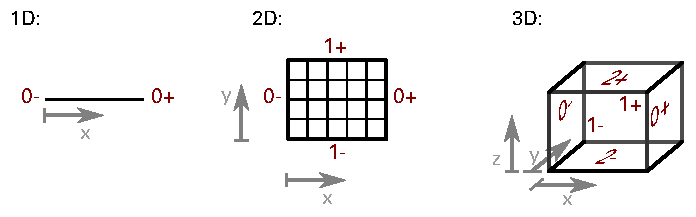
\includegraphics[width=\textwidth]{images/implementation/faces.pdf}%
  \caption{Notion of the faces of 1D, 2D and 3D elements, as used in the definition of Neumann boundary conditions.}%
  \label{fig:faces}%
\end{figure}%

For elasticity problems, where the function $f(\bfx)$ is interpreted as traction force, two more options can be set.
The first option is \code{`divideNeumannBoundaryConditionValues}\code{ByTotalArea`}. If set to \code{True}, the traction force vector is interpreted as a total force on the whole surface. The value of $T$ in \cref{eq:impl_neumann_c} is computed by scaling down the given value by the total surface area. This allows to conveniently specify a total force, which, e.g., acts on the lower end of the muscle. Without this option, the traction force is interpreted as force per area unit.

The second option \code{`isInReferenceConfiguration`} allows switching between reference and current configuration to specify the traction force. The mapping between the traction $\bfT$ in reference configuration and the traction $\bft$ in current configuration is given by the inverse deformation gradient $\bfF$:%
\begin{align}\label{eq:impl_transformation}
  \bfT = \bfF^{-1}\,\bft.
\end{align}
Because the implemented model uses the Lagrangian formulation with the right-hand side term defined in \cref{eq:impl_neumann_c}, the transformation in \cref{eq:impl_transformation} and subsequently the right-hand side have to be computed in every timestep of a dynamic problem.

\Cref{fig:traction_current_reference_configuration} illustrates the difference between Neumann boundary conditions that are specified in the  reference configuration and the current configuration. A horizontal, cuboid rod is fixed at its right end and a traction force in positive $x$ direction acts on the surface on its other end.
A dynamic hyperelasticity model with isotropic Mooney-Rivlin material is solved.

\Cref{fig:reference_configuration_1,fig:reference_configuration_2,fig:reference_configuration_3} show the simulation results, where the traction force is specified in reference configuration, \cref{fig:current_configuration_1,fig:current_configuration_2,fig:current_configuration_3} show results of the same simulation, but with the traction force specified in the current configuration.
It can be seen that the rod bends more to the right, if the traction force is specified in reference configuration. In this case, the force is always acting perpendicular to the rod, whereas, in the other version, the direction of the applied force in the global coordinate system stays constant.

\begin{figure}%
  \centering%
  \begin{subfigure}[t]{0.31\textwidth}%
    \centering%
    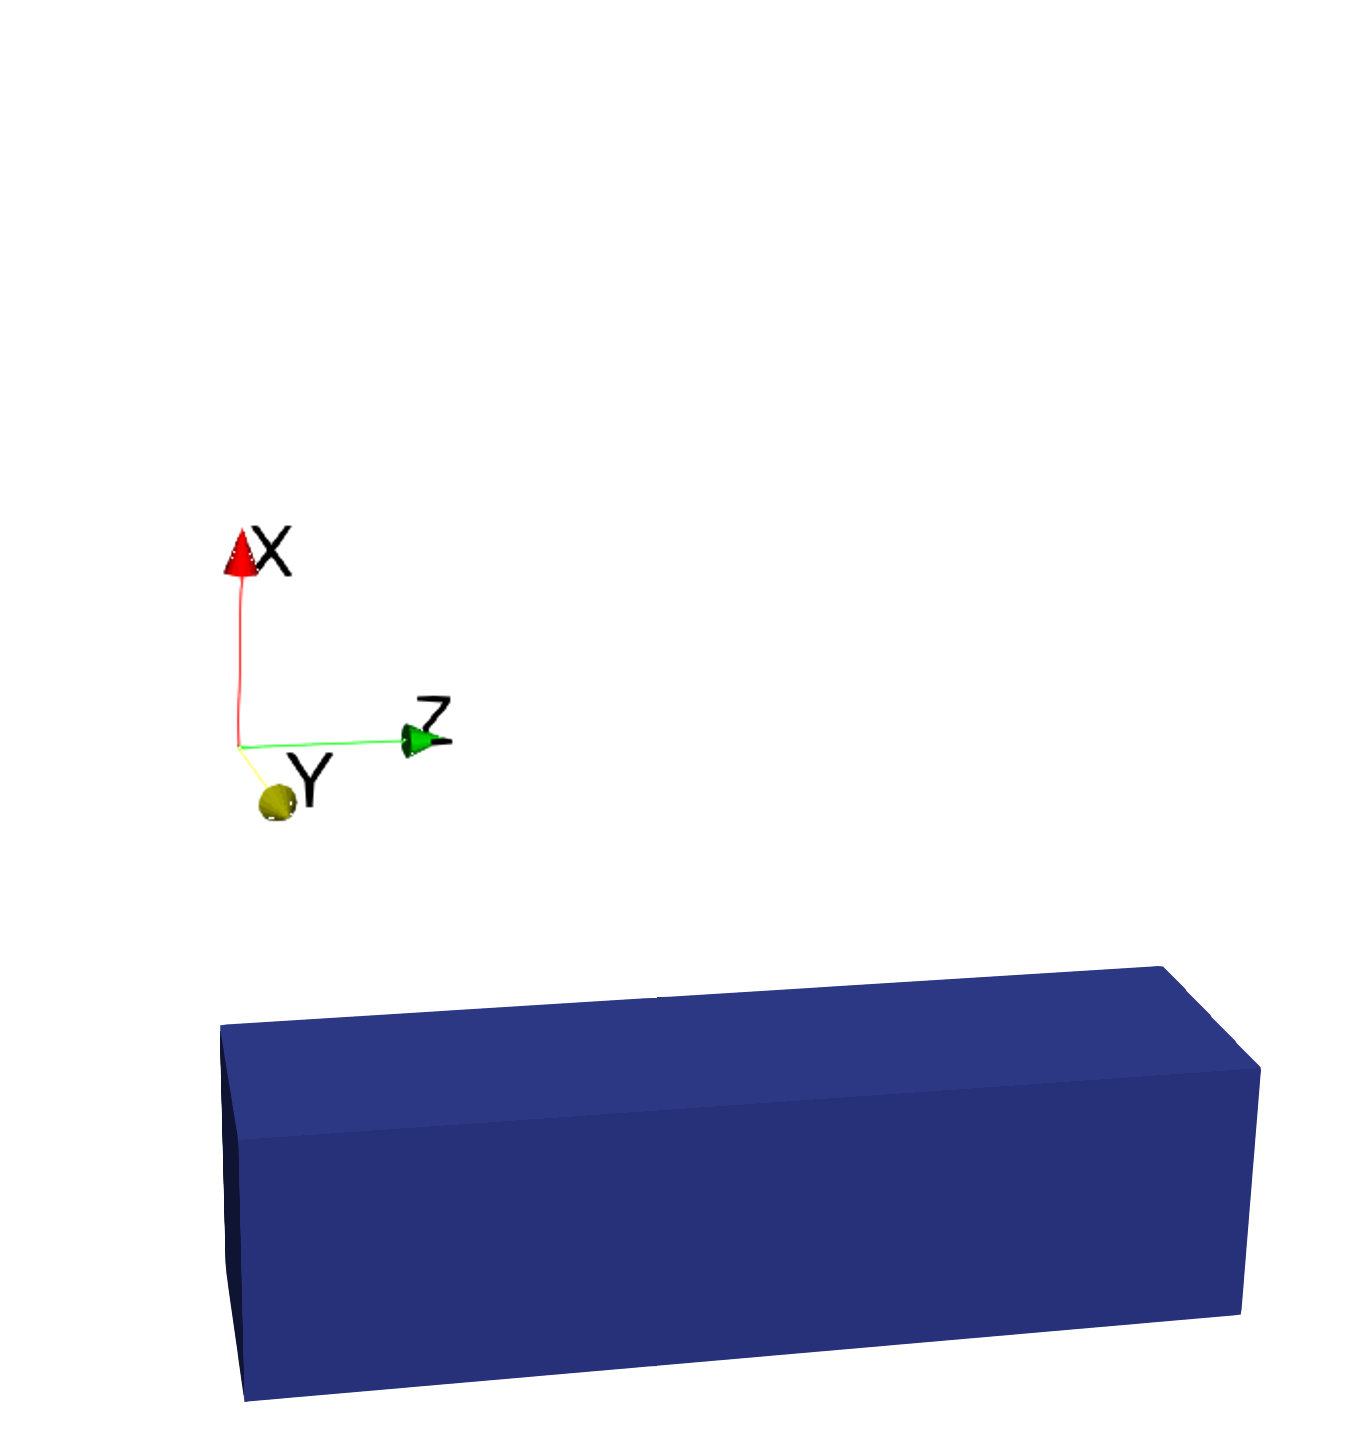
\includegraphics[width=\textwidth]{images/implementation/current_configuration_1_cropped.png}
    \caption{Boundary condition given in reference configuration, $t=\SI{1}{\milli\second}$}%
    \label{fig:reference_configuration_1}%
  \end{subfigure}
  \quad
  \begin{subfigure}[t]{0.31\textwidth}%
    \centering%
    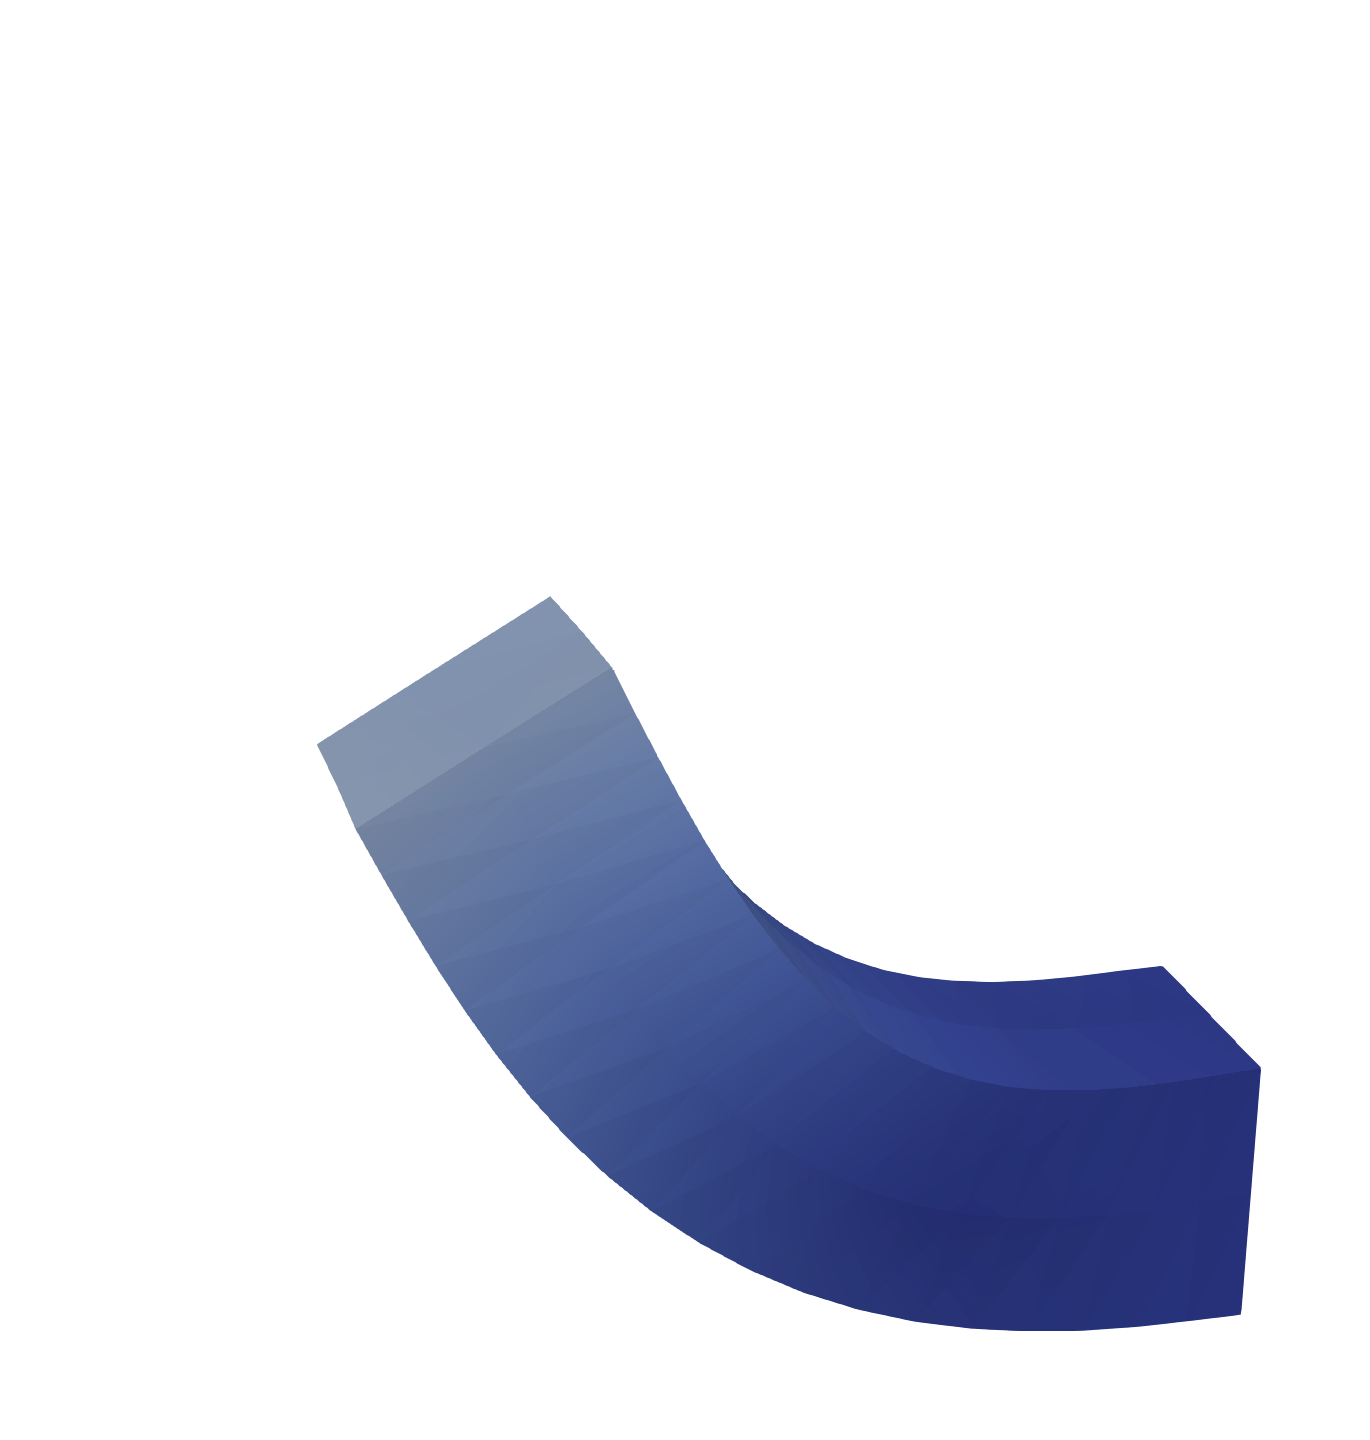
\includegraphics[width=\textwidth]{images/implementation/reference_configuration_2_cropped.png}
    \caption{Boundary condition given in reference configuration, $t=\SI{30}{\milli\second}$}%
    \label{fig:reference_configuration_2}%
  \end{subfigure}
  \quad
  \begin{subfigure}[t]{0.31\textwidth}%
    \centering%
    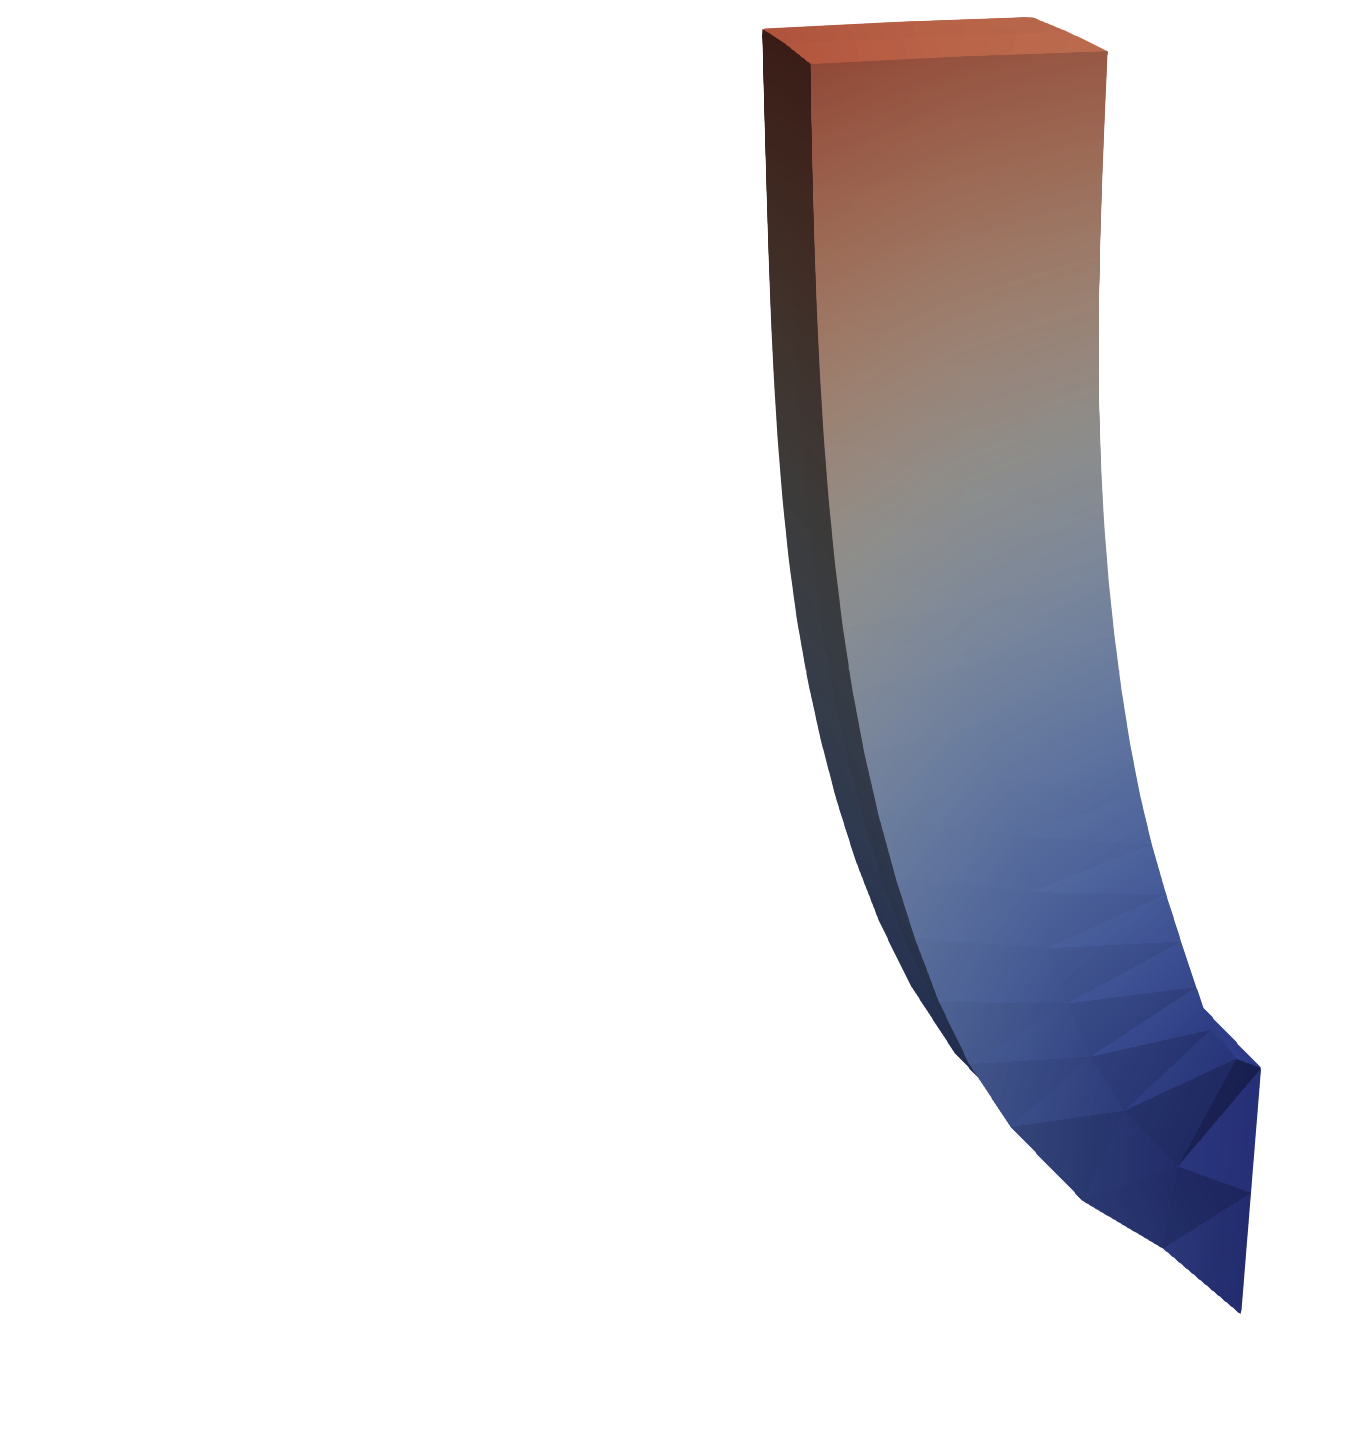
\includegraphics[width=\textwidth]{images/implementation/reference_configuration_3_cropped.png}
    \caption{Boundary condition given in reference configuration, $t=\SI{60}{\milli\second}$}%
    \label{fig:reference_configuration_3}%
  \end{subfigure}
  \\
  \begin{subfigure}[t]{0.31\textwidth}%
    \centering%
    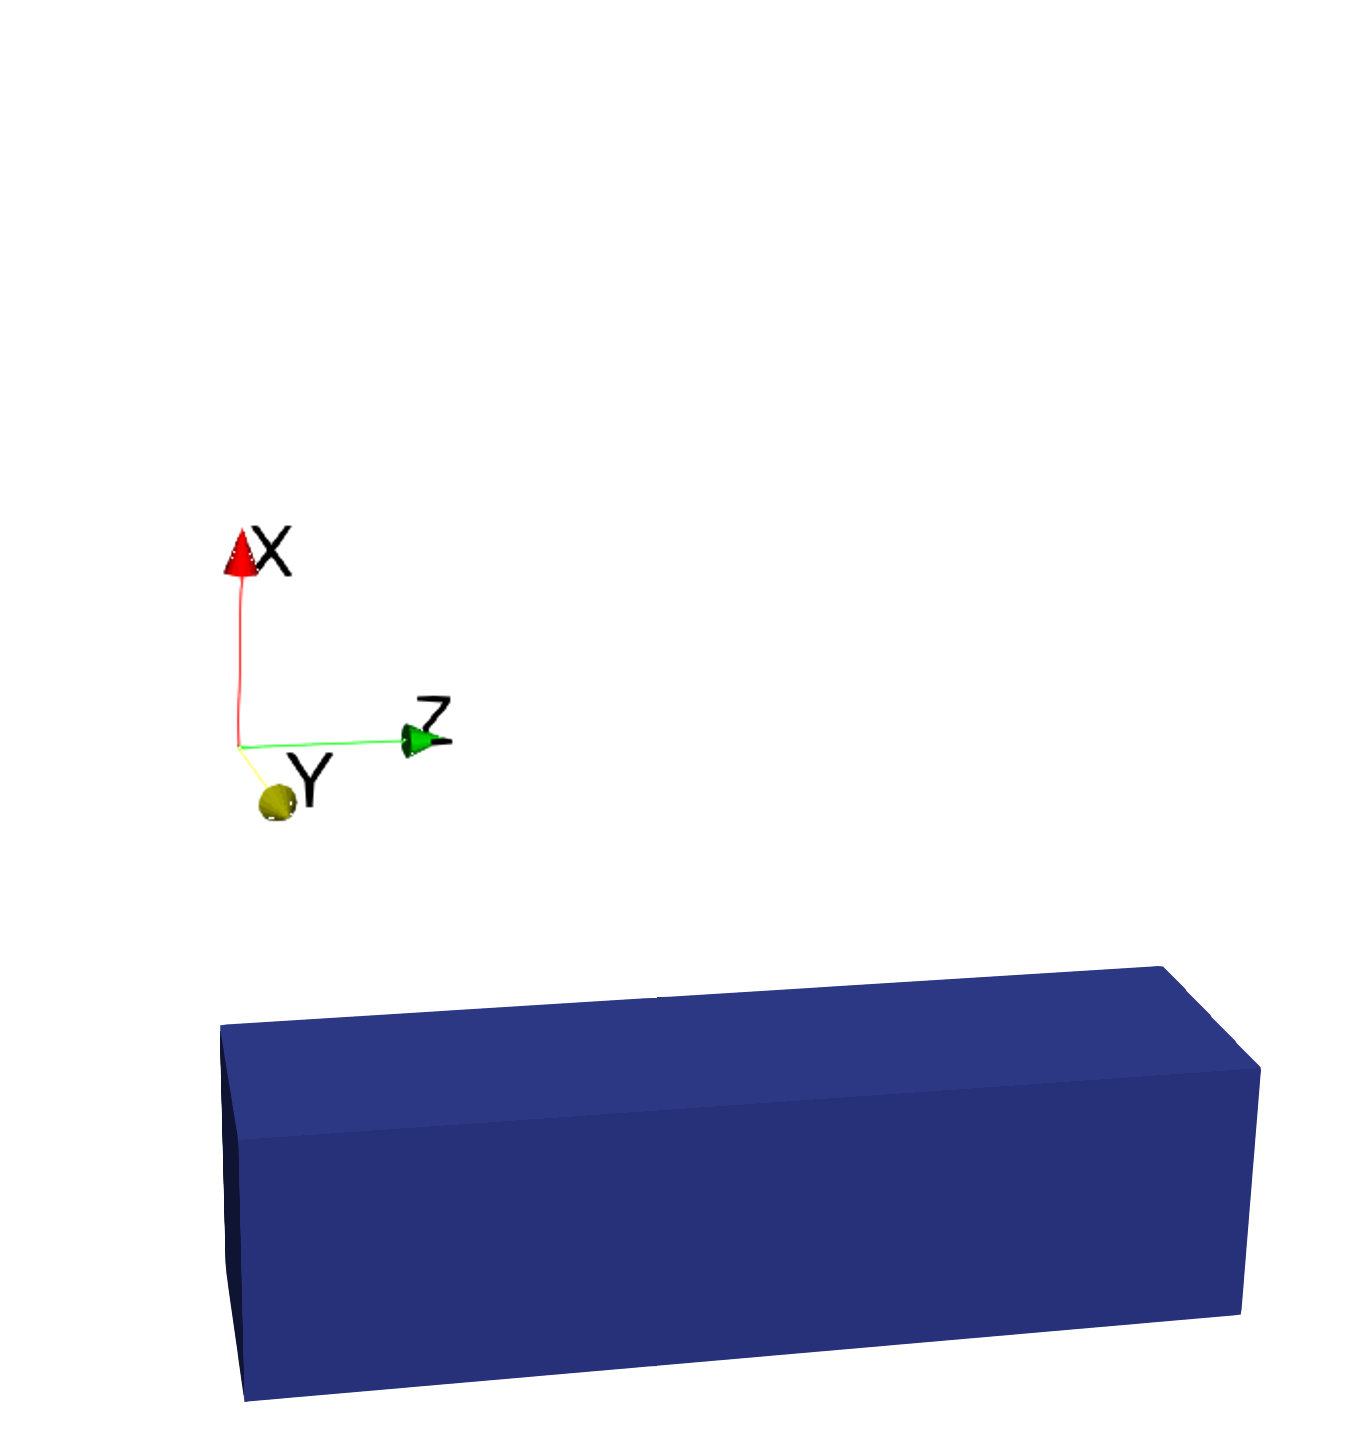
\includegraphics[width=\textwidth]{images/implementation/current_configuration_1_cropped.png}
    \caption{Boundary condition given in current configuration, $t=\SI{1}{\milli\second}$}%
    \label{fig:current_configuration_1}%
  \end{subfigure}
  \quad
  \begin{subfigure}[t]{0.31\textwidth}%
    \centering%
    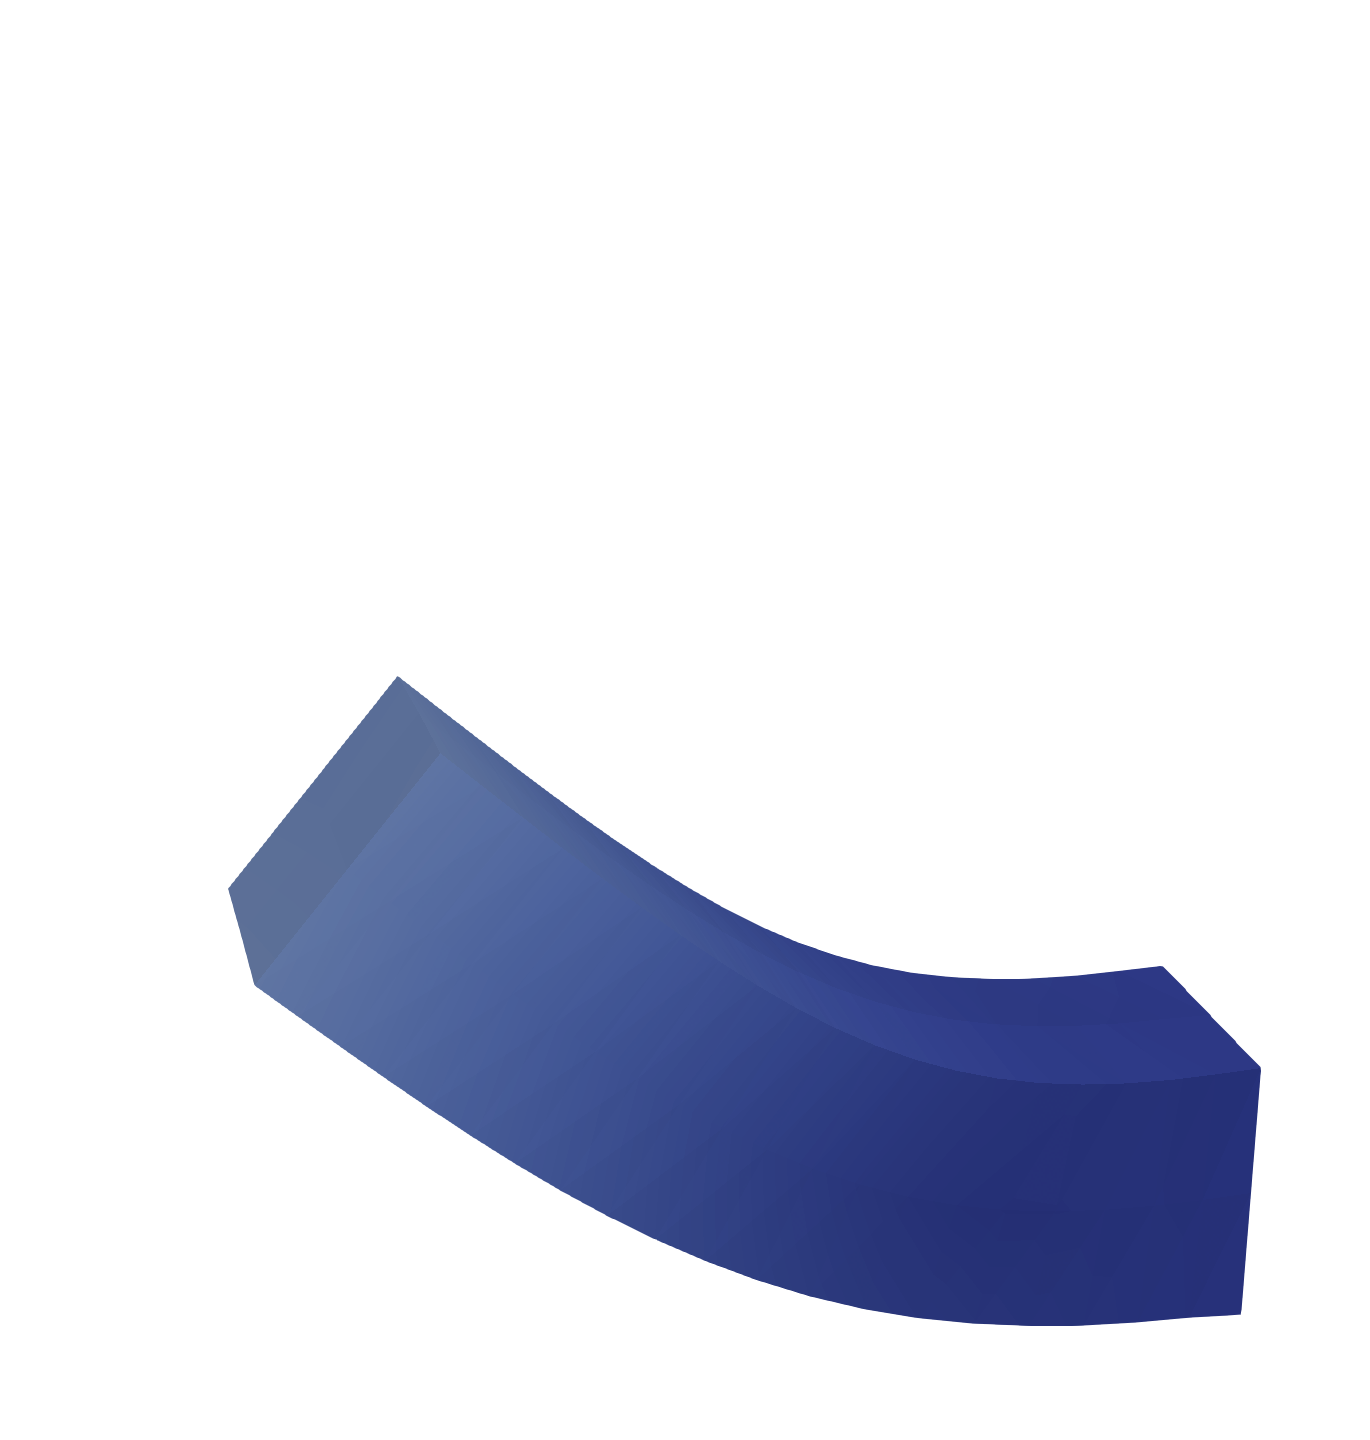
\includegraphics[width=\textwidth]{images/implementation/current_configuration_2_cropped.png}
    \caption{Boundary condition given in current configuration, $t=\SI{30}{\milli\second}$}%
    \label{fig:current_configuration_2}%
  \end{subfigure}
  \quad
  \begin{subfigure}[t]{0.31\textwidth}%
    \centering%
    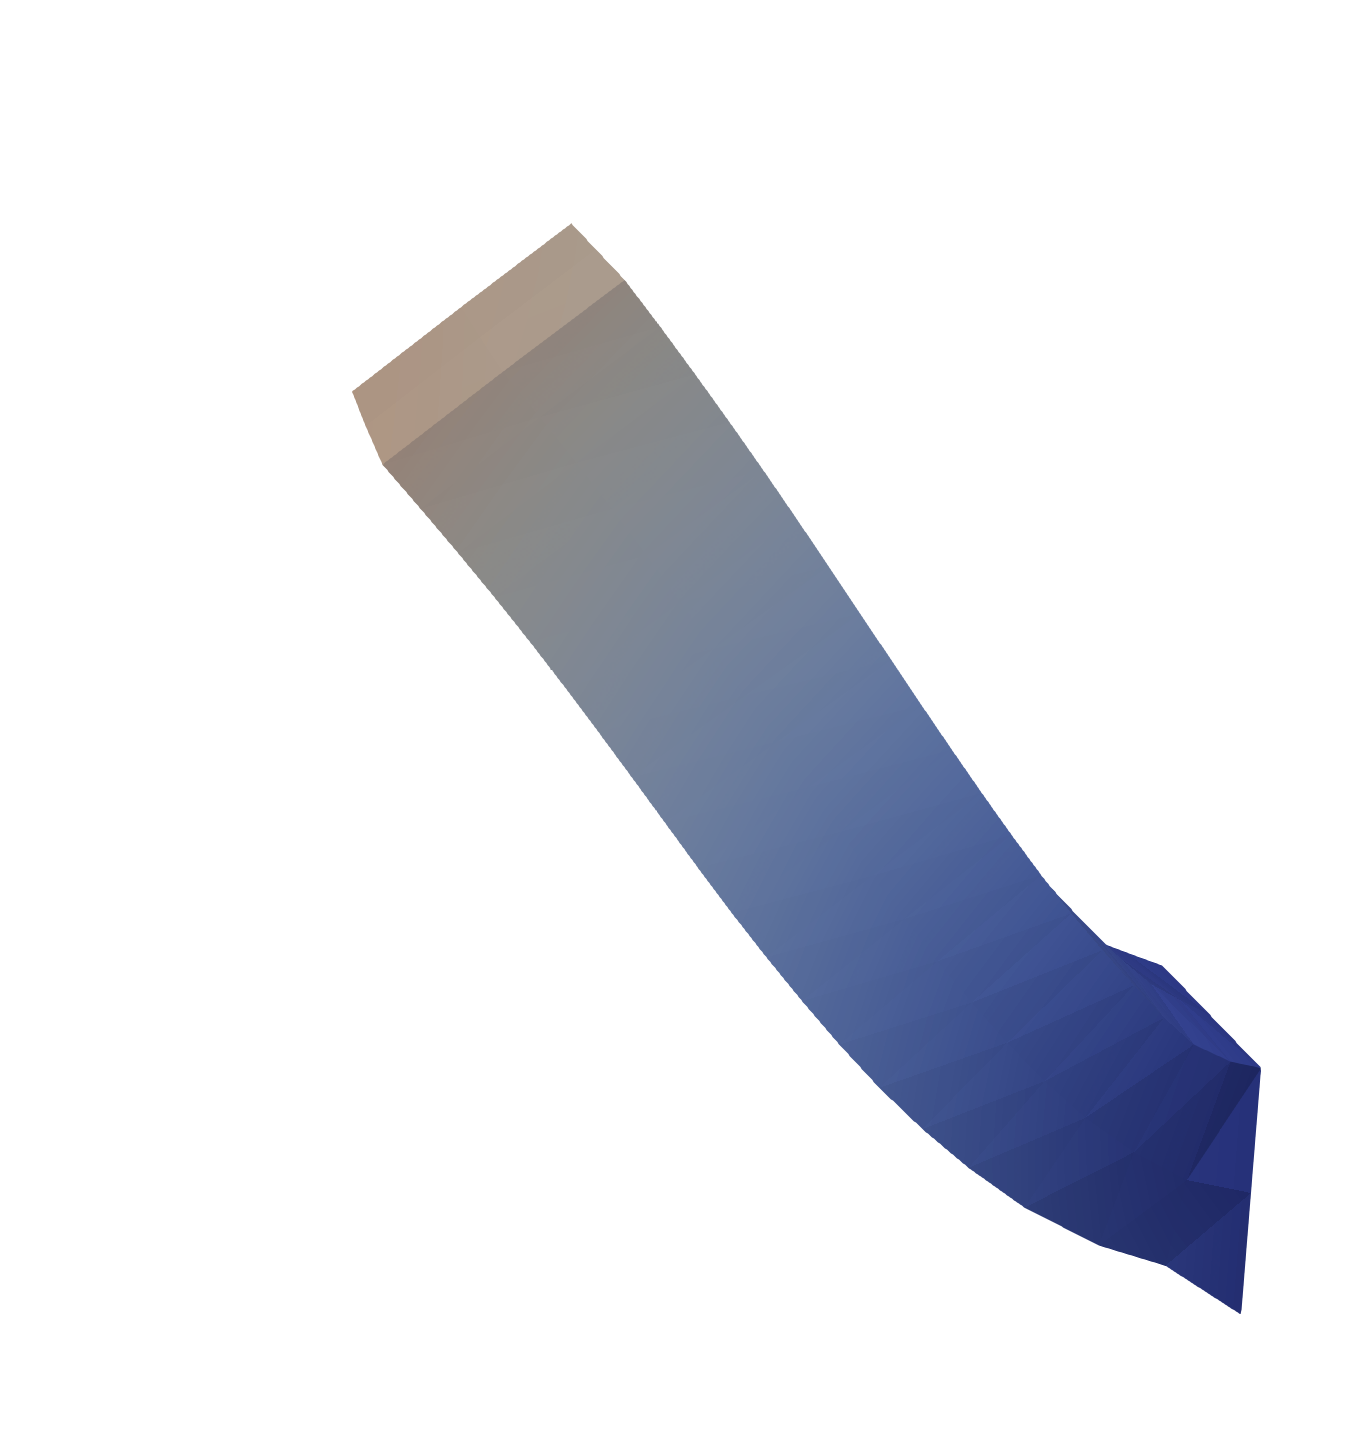
\includegraphics[width=\textwidth]{images/implementation/current_configuration_3_cropped.png}
    \caption{Boundary condition given in current configuration, $t=\SI{60}{\milli\second}$}%
    \label{fig:current_configuration_3}%
  \end{subfigure}
  \caption{Influence of whether external traction forces are defined in the current or in the reference configuration. Simulation of a dynamic solid mechanics problem with a Mooney Rivlin material model and a constant traction force in $x$ direction.}%
  \label{fig:traction_current_reference_configuration}%
\end{figure}%

\begin{reproduce}
  Use the following commands to create the results in \cref{fig:traction_current_reference_configuration}.
  \begin{lstlisting}[columns=fullflexible,breaklines=true,postbreak=\mbox{\textcolor{gray}{$\hookrightarrow$}\space}]
    cd $\$$OPENDIHU_HOME/examples/electrophysiology/fibers/fibers_contraction/with_tendons_precice/meshes
    ./create_cuboid_meshes.sh     # create the cuboid mesh
    cd $\$$OPENDIHU_HOME/examples/electrophysiology/fibers/fibers_contraction/with_tendons_precice/traction_current_or_reference_configuration
    mkorn && srr       # build
    ./muscle_precice settings_current_configuration.py ramp.py
    ./muscle_precice settings_reference_configuration.py ramp.py
  \end{lstlisting}
\end{reproduce}


% matrices? how they are stored in PETSc, different approaches in elasticity and multidomain -> no
% slot connector data and transfer, no already described

